\chapter{Numerical Calculus}
In this chapter we discuss techniques for approximating the two primary computations
in calculus: taking derivatives and evaluating definite integrals. Throughout this chapter
we will make heavy use of Taylor's Theorem to build these approximations. At the end of
the chapter we'll examine a numerical technique for solving optimization problems without
explicitly finding derivatives. 

\section{Differentiation}
In this section we'll build several approximation of first and second derivatives.  The
idea for each of these approximation is:
\begin{itemize}
    \item Partition the interval $[a,b]$ into $N$ points.
    \item Approximate the derivative at the point $x \in [a,b]$ by using linear
        combinations of $f(x-h)$, $f(x)$, $f(x+h)$, and/or other points in the partition.  
\end{itemize}
Partitioning the interval into discrete points turns the continuous problem of finding a
derivative at every real point in $[a,b]$ into a discrete
problem where we calculate the approximate derivative at finitely many points in $[a,b]$.
Figure \ref{fig:differentiation_partition} shows a depiction of the partition as well as
making clear that $h$ is the separation between each of the points in the partition.  Note
that in general the points in the partition do not need to be equally spaced, but that is
the simplest place to start.
\begin{figure}[ht!]
    \begin{center}
        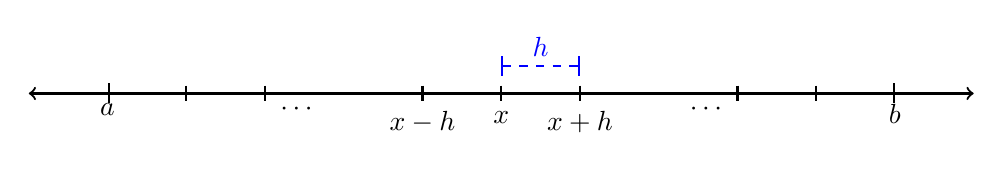
\begin{tikzpicture}
            \draw[<->, thick] (-1,0) -- (11,0);
            \draw[|-|,thick] (0,0) node[anchor=north]{$a$} -- (10,0)
            node[anchor=north]{$b$};
            \foreach \j in {1,2,8,9}{
                \draw[thick] (\j,0.1) -- (\j,-0.1);
            }
            \draw (2.4,0) node[anchor=north]{$\cdots$};
            \draw (7.6,0) node[anchor=north]{$\cdots$};
            \draw[thick] (4.0,0.1) -- (4,-0.1) node[anchor=north]{$x-h$};
            \draw[thick] (5,0.1) -- (5,-0.1) node[anchor=north]{$x$};
            \draw[thick] (6.0,0.1) -- (6,-0.1) node[anchor=north]{$x+h$};
            \draw[dashed, blue, thick,|-|] (5,0.35) -- (6,0.35);
            \draw[blue] (5.5,0.35) node[anchor=south]{$h$};
        \end{tikzpicture}
    \end{center}
    \caption{A partition of an interval on the real line.}
    \label{fig:differentiation_partition}
\end{figure}

If we recall that the definition of the first derivative of a function is
\begin{flalign}
    \frac{df}{dx} = \lim_{h \to 0} \frac{f(x+h) - f(x)}{h}.
    \label{eqn:derivative_defintiion}
\end{flalign}
our first approximation for the first derivative is naturally
\begin{flalign}
    \frac{df}{dx} \approx \frac{f(x+h) - f(x)}{h}.
    \label{eqn:derivative_first_approx}
\end{flalign}
In \eqref{eqn:derivative_first_approx} we have simply removed the limit and instead
approximated the derivative as the slope.  It should be clear that this approximation is
only good if $h$ is {\it small}.  The linear combination that we
spoke about before is
\[ \frac{df}{dx} \approx \frac{1}{h} f(x+h) - \frac{1}{h} f(x). \]
While this is the simplest and most obvious approximation for the first derivative there
is a much more elegant technique, using Taylor series, for arriving at this approximation.
Furthermore, the Taylor series technique suggests an infinite family of other techniques.


\begin{problem}\label{prob:numdiff1}
    From Taylor's Theorem we know that for an infinitely differentiable function $f(x)$,
    \[ f(x) = f(a) + \frac{f'(a)}{1!} (x-a)^1 + \frac{f''(a)}{2!}(x-a)^2 +
        \frac{f^{(3)}(a)}{3!}(x-a)^3 + \frac{f^{(4)}(a)}{4!}(x-a)^4 + \cdots. \] 
    What do we get if we replace $x$ with $x+h$ and $a$ with $x$?  In other words, in
    Figure \ref{fig:differentiation_partition} we want to center the Taylor series at $x$
    and evaluate the resulting series at the point $x+h$.
    \[ f(x+h) = \underline{\hspace{3in}} \]
\end{problem}


\begin{problem}\label{prob:num_diff_first_order}
    Solve the result from the previous problem for $f'(x)$ to create an approximation for
    $f'(x)$ using $f(x+h)$, $f(x)$, and some higher order terms. (fill in the blanks and
    the question marks)
    \[ f'(x) = \frac{f(x+h) - ???}{??} + \underline{\hspace{1in}} \]
\end{problem}
\solution{
    \begin{flalign*}
        f(x+h) &= f(x) + \frac{f'(x)}{1!}(x+h-x) + \frac{f''(x)}{2!}h^2 + \cdots \\
        f'(x) &= \frac{f(x+h)-f(x)}{h} + \frac{f''(\xi)}{2} h \quad \text{for} \quad \xi
        \in (x,x+h)
    \end{flalign*}
    The error is on the order of $h$.
}

\begin{problem}
    If we were to drop everything after the fraction in the previous problem we know that
    we would be introducing error into our derivative computation.  According to Taylor's
    Theorem, how can we quantify the error of the approximation?
\end{problem}

\begin{definition}[Order of a Numerical Derivative]
    The {\bf order} of a numerical derivative is the power of the step size in the
    remainder term.  For example, a first order method will have ``$h^1$'' in the
    remainder term.  A second order method will have ``$h^2$'' in the remainder term.
\end{definition}

\begin{thm}[First Order Approximation of the First
    Derivative]\label{thm:first_order_first_deriv}
    In problem \ref{prob:num_diff_first_order} we derived a first order approximation of
    the first derivative:
    \[ f'(x) = \frac{f(x+h) - f(x)}{h} + \mathcal{O}(h). \]
    In this formula, $h = \Delta x$ is the step size.
\end{thm}
In the previous definition, ``$\mathcal{O}(h)$'' (read: big-O of $h$) states that the
method is first order.  This means that the maximum error that you're making with this
method is on the order of the size of the step.  Not surprisingly, if we let $h$ get
arbitrarily small then the error in this method gets arbitrarily small.  More formally we
have the following definition.

\begin{definition}[Big $\mathcal{O}$ Notation]
    We say that the error in a differentiation method is ``big O of $h$'', $E =
    \mathcal{O}(h)$, if and only if there is a positive constant $M$ such that 
    \[ |Error| \le M |h|. \]
    This is equivalent to saying that a differentiation method is first order.
\end{definition}

\begin{problem}
    Explain what the phrase
    \begin{quote}
        {\it ``The approximation of $f'(x)$ in Theorem \ref{thm:first_order_first_deriv} is $\mathcal{O}(h)$''}
    \end{quote}
    into your own words.  
\end{problem}


\begin{problem}\label{prob:deriv_error_analysis_ex}
   Consider the function $f(x) = \sin(x) - x\sin(x)$.  The goal of this problem is to make
   sense of the discussion of the ``order'' of the derivative approximation.  You may want
   to pause first and reread the previous couple of pages.
   \begin{enumerate}
       \item[(a)] Find $f'(x)$ by hand.
       \item[(b)] Use your answer to part (a) to verify that $f'(1) = -\sin(1) \approx
           -0.8414709848$.  
       \item[(c)] To approximate the first derivative at $x=1$ numerically we calculate 
           \[ f'(1) \approx \frac{f(1+h) - f(1)}{h}. \]
           Fill in the table below with the derivative approximation and the absolute
           error associated with each given $h$.  You may want to use a spreadsheet to
           organize your data (be sure that you're working in radians!).
           \begin{center}
               \begin{tabular}{|c|c|c|c|}
                   \hline 
                   $h$ & Approx. of $f'(1)$ & Exact value of $f'(1)$ & Abs.
                   \% Error \\ \hline \hline
                   $2^{-3} = 0.125$ & & $-\sin(1)$ & \\ \hline
                   $2^{-4}=0.0625$ & & $-\sin(1)$ & \\ \hline
                   $2^{-5}$ & & $-\sin(1)$ & \\ \hline
                   $2^{-6}$ & & $-\sin(1)$ & \\ \hline
                   $2^{-7}$ & & $-\sin(1)$ & \\ \hline
                   $2^{-8}$ & & $-\sin(1)$ & \\ \hline
                   $2^{-9}$ & & $-\sin(1)$ & \\ \hline
               \end{tabular}
           \end{center}
       \item[(d)] There was nothing really special in part (c) about powers of 2.  Use
           your spreadsheet to build similar tables for the following sequences of $h$:
       \begin{flalign*}
           h &= 3^{-1}, \, 3^{-2}, \, 3^{-3}, \, \ldots \\
           h &= 5^{-1}, \, 5^{-2}, \, 5^{-3}, \, \ldots \\
           h &= 10^{-1}, \, 10^{-2}, \, 10^{-3}, \, \ldots \\
           h &= \pi^{-1}, \, \pi^{-2}, \, \pi^{-3}, \, \ldots \\
        \end{flalign*}
       \item[(e)] Observation: If you calculate a numerical derivative with a forward
           difference and then calculate the absolute percent error with a fixed value of
           $h$, then what do you expect to happen to the absolute error if you divide the
           value of $h$ by some positive contant $M$?
       \item[(f)] What does your answer to part (e) have to do with the approximation
           order of the numerical derivative method that you used?
   \end{enumerate}
\end{problem}

\begin{problem}
    Assume that $f(x)$ is some differentiable function and that we have calculated the
    value of $f'(c)$ using the forward difference formula
    \[ f'(c) \approx \frac{f(c+h) - f(c)}{h}. \]
    Using what you learned from the previous problem to fill in the following table.
    \begin{center}
        \begin{tabular}{|c|c|}
            \hline 
            My $h$ & Absolute Percent Error \\ \hline \hline
            $0.2$ & $2.83\%$ \\ \hline
            $0.1$ & \\ \hline
            $0.05$ & \\ \hline
            $0.02$ & \\ \hline
            $0.002$ & \\ \hline
        \end{tabular}
    \end{center}
\end{problem}

\begin{problem}
    Write \ProgLang code that takes a function and a domain $(xmin,xmax)$ and
    returns a numerical approximation to the derivative on the interval
    $(xmin,xmax)$. You should ALWAYS start by writing pseudo-code as comments in your
    \ProgLang file.   Your function should accept \ifnum\Python=0 an anonymous function
    handle\else a Python function\fi, the
    bounds on the domain, and the number of interior points used for approximation within
    the domain.  Your function should output the $x$ values and $y$ values associated with
    the derivative.\\
    \ifnum\Python=0
    \mcode{function [newx,yprime]=FirstDerivFirstOrder(f,xmin,xmax,num_interior_pts)} 
    \else
    \mcode{def FirstDerivFirstOrder(f,xmin,xmax,num_interior_pts):} 
    \fi
\end{problem}

The only two ways to really check a numerical derivative are to plot the numerical
approximation and to do the derivative by hand and to plot the error. Be warned, however,
that the numerical derivative that we have built from Theorem
\ref{thm:first_order_first_deriv} should have one less value than the
original list of $x$ and $y$ values.  Think about why this must be true. Also double check
your code from the previous problem and make sure that you can plot \mcode{newx} vs
\mcode{yprime} without having to change their size.  

\begin{example}[Efficient Coding with Vectors]
Let's pause now for a few words on efficient vector-based coding.  We can absolutely write
code for the first derivative using a \mcode{for} loop as you can see in the code below.
Notice that I have resized the $x$ vector so that it is the same length as the $y'$ vector.

\bcode
\ifnum\Python=0
\begin{lstlisting}
function [newx,yprime] = FirstDerivFirstOrder(f,xmin,xmax,num_interior_pts)
    x = linspace(xmin,xmax,num_interior_pts))
    y = f(x)
    yprime = zeros(length(y)-1)
    newx = zeros(length(x)-1)
    for n = 1:length(yprime)
        newx(n) = x(n)
        yprime(n) = (y(n+1)-y(n)) / (x(n+1) - x(n))
    end
end
\end{lstlisting}
\else
\begin{lstlisting}
def FirstDerivFirstOrder(f,xmin,xmax,num_interior_pts):
    import numpy as np
    x = np.array(np.linspace(xmin,xmax,num_interior_pts))
    y = f(x)
    yprime = np.zeros(y.size-1)
    newx = np.zeros_like(yprime)
    for n in range(0,y.size-1):
        newx[n] = x[n]
        yprime[n] = (y[n+1]-y[n]) / (x[n+1] - x[n])
    return(newx, yprime)
\end{lstlisting}
\fi

Implementing this code we can use the following script.

\bcode
\ifnum\Python=0
\begin{lstlisting}
f = @(x) sin(x)
xmin = 0
xmax = 2*pi
numpts = 100
x = linspace(xmin,xmax,numpts)
y = f(x)
[newx, yprime] = FirstDerivFirstOrder(f,xmin,xmax,numpts)
plot(x,y,'b--',newx,yprime,'r--')
grid on
\end{lstlisting}
\else
\begin{lstlisting}
import matplotlib.pyplot as plt
import numpy as np
%matplotlib inline # for use in Jupyter Notebooks

def f(x): # define the function of interest
    import numpy as np
    return(np.sin(x))
xmin = 0
xmax = 2*np.pi
numpts = 100
x = np.linspace(xmin,xmax,numpts)
y = f(x)
dx, dy = FirstDerivFirstOrder(f,xmin,xmax,numpts)
plt.plot(x,y,'b--',newx,yprime,'r--')
plt.grid()
\end{lstlisting}
\fi
The output of this code will give the sine function along with the derivative, the cosine
function as seen in Figure \ref{fig:first_deriv_sine}.

Now let's build the first derivative function in a much smarter way.  Instead of looping
over all of the elements we can take advantage of the fact that every thing is stored in
vectors.  Hence we can just do vector operations and do all of the subtractions and
divisions at once.
\ifnum\Python=0
\begin{lstlisting}
function [newx, yprime] = FirstDerivFirstOrder(f,xmin,xmax,num_interior_pts)
    x = linspace(xmin,xmax,num_interior_pts);
    y = f(x);
    yprime = (y(2:end) - y(1:end-1)) ./ (x(2:end) - x(1:end-1));
    newx = x(1:end-1)
end
\end{lstlisting}
\else
\begin{lstlisting}
def FirstDerivFirstOrder(f,xmin,xmax,num_interior_pts):
    import numpy as np
    x = np.array(np.linspace(xmin,xmax,num_interior_pts))
    y = f(x)
    yprime = (y[1:]-y[:-1]) / (x[1:] - x[:-1])
    newx = x[:-1]
    return(newx, yprime)
\end{lstlisting}
\fi


\end{example}

\begin{figure}[ht!]
    \begin{center}
        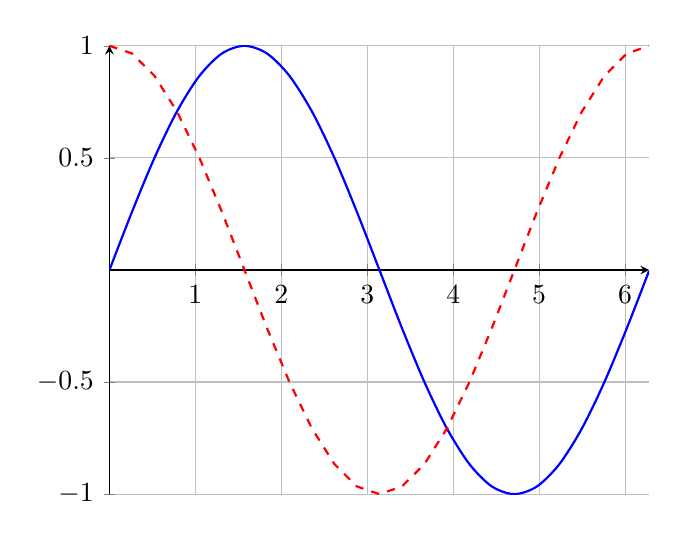
\begin{tikzpicture}
            \begin{axis}[axis lines=center, grid, domain=0:6.28]
                \addplot[smooth, thick, blue] {sin(deg(x))};
                \addplot[dashed, thick, red] {cos(deg(x))};
            \end{axis}
        \end{tikzpicture}
    \end{center}
    \caption{The result of using the first derivative code with 100 interior point on the
    function $f(x) = \sin(x)$.}
    \label{fig:first_deriv_sine}
\end{figure}


\begin{problem}
    Write code that finds a first order approximation for the first derivative
    of $f(x) = \sin(x) - x\sin(x)$ on the interval $x \in (0,15)$.  Your script should
    output two plots (side-by-side). 
    \begin{enumerate}
        \item The left-hand plot should show the function in blue and the first derivative
            as a red dashed curve. Sample code for this problem is
           \ifnum\Python=0
\begin{lstlisting}
 f = @(x) sin(x) - x*sin(x);
 a=0; b=15;
 num_interior_pts = 1000; % this should be LARGE
 x = linspace(a,b,num_interior_pts);
 [new_x,dfdx] = FirstDerivFirstOrder(f,a,b,num_interior_pts);
 subplot(1,2,1)
 plot(x, f(x) , 'b' , new_x , dfdx , 'r--')
\end{lstlisting}
\else
\begin{lstlisting}
import matplotlib.pyplot as plt
import numpy as np
%matplotlib inline
def f(x):
    import numpy as np
    return(np.sin(x) - x * np.sin(x))
xmin = 0
xmax = 15
numpts = 1000
x = np.linspace(xmin,xmax,numpts)
y = f(x)
newx, yprime = FirstDerivFirstOrder(f,xmin,xmax,numpts)

fig, ax = plt.subplots(1,2)
ax[0].plot(x,y,'b',newx,yprime,'r--')
ax[0].grid()
\end{lstlisting}
\fi
        \item The right-hand plot should show the absolute error between the exact
            derivative and the numerical derivative.  You should use a logarithmic $y$
            axis for this plot.
            \ifnum\Python=0
\begin{lstlisting}
df = @(x) ... % write code for the exact derivative
subplot(1,2,2)
plot(new_x, abs( df(new_x) - dfdx ) , 'k--')
\end{lstlisting}
\else
\begin{lstlisting}
def df(x):
    # write a function for the exact derivative
dy = df(newx)
ax[1].semilogy(newx,abs(dy - yprime))
ax[1].grid()
\end{lstlisting}
\fi
    \end{enumerate}
    Discuss how you can see the fact that this is a first order method.  You may want to
    put one (or both) of the plots on a log-log scale or a semi-log scale \ldots I'll let
    you figure out which one makes the most sense.
\end{problem}


Let's return to the mathematics: \\
Next we'll build a more accurate numerical first derivative scheme.  The derivation
technique is the same: play a little algebra game with the Taylor series and see if you
can get the first derivative to simplify out.  This time we'll be hoping to have a better
error approximation.

\begin{problem}\label{prob:numdiff3}
    Consider again the Taylor series for an infinitely differentiable function $f(x)$:
    \[ f(x) = f(a) + \frac{f'(a)}{1!} (x-a)^1 + \frac{f''(a)}{2!}(x-a)^2 +
        \frac{f^{(3)}(a)}{3!}(x-a)^3 + \frac{f^{(4)}(a)}{4!}(x-a)^4 + \cdots \] 
    \begin{enumerate}
        \item[(a)] This time, replace $x$ with $x-h$ and $a$ with $x$ and simplify.  
            \[ f(x-h) = \underline{\hspace{3in}} \]
        \item[(b)] You should already have the Taylor series for $f(x+h)$.  Subtract
            $f(x+h)$ and $f(x-h)$ and simplify.  Be very careful of you signs.  
            \[ f(x+h) - f(x-h) = \underline{\hspace{3in}} \]
        \item[(c)] Solve for $f'(x)$ in your result from part (b).  Fill in the question
            marks and blanks below once you have finished simplifying.
            \[ f'(x) = \frac{(???) - (???)}{2h} + \underline{\hspace{1in}}. \]
    \end{enumerate}
\end{problem}

\begin{problem}
    If we were to drop the terms after the fraction in the last result then we would be
    making an error in the derivative computation.  According to Taylor's Theorem quantify
    the error that is being made.
\end{problem}

\begin{thm}[Second Order Approximation of the First Derivative]
    \[ f'(x) = \underline{\hspace{2in}} + \mathcal{O}(h^2) \]
\end{thm}


\begin{problem}
    Let's return to the function $f(x) = \sin(x) - x\sin(x)$ but this time we will
    approximate the first derivative at $x=1$ using the formula
    \[ f'(1) \approx \frac{f(1+h) - f(1-h)}{2h}. \]
    You should already have the first derivative and the exact answer from Problem
    \ref{prob:deriv_error_analysis_ex} (if not, then go get them by hand again).  
    \begin{enumerate}
        \item[(a)] Fill in the table below with the derivative approximation and the absolute
           error associated with each given $h$.  You may want to use a spreadsheet to
           organize your data (be sure that you're working in radians!).
           \begin{center}
               \begin{tabular}{|c|c|c|c|}
                   \hline 
                   $h$ & Approx. of $f'(1)$ & Exact value of $f'(1)$ & Abs.
                   \% Error \\ \hline \hline
                   $2^{-3} = 0.125$ & & $-\sin(1)$ & \\ \hline
                   $2^{-4}=0.0625$ & & $-\sin(1)$ & \\ \hline
                   $2^{-5}$ & & $-\sin(1)$ & \\ \hline
                   $2^{-6}$ & & $-\sin(1)$ & \\ \hline
                   $2^{-7}$ & & $-\sin(1)$ & \\ \hline
                   $2^{-8}$ & & $-\sin(1)$ & \\ \hline
                   $2^{-9}$ & & $-\sin(1)$ & \\ \hline
               \end{tabular}
           \end{center}
       \item[(b)] There was nothing really special in part (c) about powers of 2.  Use
           your spreadsheet to build similar tables for the following sequences of $h$:
       \begin{flalign*}
           h &= 3^{-1}, \, 3^{-2}, \, 3^{-3}, \, \ldots \\
           h &= 5^{-1}, \, 5^{-2}, \, 5^{-3}, \, \ldots \\
           h &= 10^{-1}, \, 10^{-2}, \, 10^{-3}, \, \ldots \\
           h &= \pi^{-1}, \, \pi^{-2}, \, \pi^{-3}, \, \ldots 
        \end{flalign*}
       \item[(c)] Observation: If you calculate a numerical derivative with a centered
           difference and calculate the resulting absolute percent error with a fixed
           value of $h$, then what do you expect to happen to the absolute percent error
           if you divide the value of $h$ by some positive contant $M$?
       \item[(d)] What does your answer to part (e) have to do with the approximation
           order of the numerical derivative method that you used?
    \end{enumerate}
\end{problem}


\begin{problem}
    Assume that $f(x)$ is some differentiable function and that we have calculated the
    value of $f'(c)$ using the centered difference formula
    \[ f'(c) \approx \frac{f(c+h) - f(c-h)}{2h}. \]
    Using what you learned from the previous problem to fill in the following table.
    \begin{center}
        \begin{tabular}{|c|c|}
            \hline 
            My $h$ & Absolute Percent Error \\ \hline \hline
            $0.2$ & $2.83\%$ \\ \hline
            $0.1$ & \\ \hline
            $0.05$ & \\ \hline
            $0.02$ & \\ \hline
            $0.002$ & \\ \hline
        \end{tabular}
    \end{center}
\end{problem}


\begin{problem}
    Write a \ProgLang function that takes a function and a domain and returns a second order
    numerical approximation to the first derivative on the interval. You should ALWAYS start by writing pseudo-code as comments in your
    \ProgLang file.    Your function should
    accept a function, the bounds on the domain, and the number of
    interior points used for approximation within the domain. Your function should output
    the x values and y values associated with the derivative.\\
    \ifnum\Python=0
    \mcode{function [new_x,dfdx]=FirstDerivSecondOrder(f,xmin,xmax,num_interior_pts)}
    \else
    \mcode{def FirstDerivSecondOrder(f,xmin,xmax,num_interior_pts):}
    \fi
    You should try to write this code without using any \mcode{for} loops.
\end{problem}

Now we'll search for an approximation of the second derivative.  Again, the game will be
the same: play with the Taylor series and some algebra and hope that the second derivative
pops out.  This time we'll do the algebra in such a way that the first derivative cancels.

From the previous problems you already have Taylor expansions of the form $f(x+h)$ and
$f(x-h)$.  Let's summarize them here since you're going to need them for future
computations.
\begin{flalign*}
    f(x+h) &= f(x) + \frac{f'(x)}{1!} h + \frac{f''(x)}{2!} h^2 + \frac{f^{(3)}(x)}{3!}
    h^3 + \cdots \\
    f(x-h) &= f(x) - \frac{f'(x)}{1!} h + \frac{f''(x)}{2!} h^2 - \frac{f^{(3)}(x)}{3!}
    h^3 + \cdots 
\end{flalign*}

\begin{problem}\label{prob:numdiff4}
    The goal of this problem is to use the Taylor series for $f(x+h)$ and $f(x-h)$ to arrive at an approximation of the
    \underline{ {\bf second derivative}}. 
    \begin{enumerate}
        \item[(a)] Add the Taylor series for $f(x+h)$ and $f(x-h)$ and combine all like
            terms.  You should notice that several terms cancel.
            \[ f(x+h) + f(x-h) = \underline{\hspace{3in}}. \]
        \item[(b)] Solve your answer in part (a) for $f''(x)$.
            \[ f''(x) = \frac{(??) - 2 (??) + (??)}{h^2} + \underline{\hspace{1in}}. \]
    \end{enumerate}
\end{problem}

\begin{problem}
    If we were to drop all of the terms after the fraction on the right-hand side of the
    previous result we would be introducing some error into the derivative computation.
    According to Taylor's Theorem, how can we quantify the order of the error?  
\end{problem}

\begin{problem}
    Again consider the function $f(x) = \sin(x) - x\sin(x)$. 
    \begin{enumerate}
        \item[(a)] Calculate the \underline{second} derivative of this function and
            calculate the exact value of $f''(1)$.
        \item[(b)] If we calcuate the second derivative with the central difference scheme
            that you built in the Problem \ref{prob:numdiff4} using $h = 0.5$ then we get
            a 4.115\% error.  Stop now and verify this percent error calculation.  
        \item[(c)] Based on our previous work with the order of the error in a numerical
            differentiation scheme, what do you predict the error will be if we calculate
            $f''(1)$ with $h = 0.25$?  With $h = 0.05$?  With $h = 0.005$?  Be able to
            defend your answers.
    \end{enumerate}
\end{problem}



\begin{problem}
    Write a \ProgLang function that takes a function and a domain and returns a second order
    numerical approximation to the second derivative on the interval. You should ALWAYS start by writing pseudo-code as comments in your
    \ProgLang file.    Your function should
    accept a function, the bounds on the domain, and the number of
    interior points used for approximation within the domain. Your function should output
    the x values and y values associated with the derivative.\\
    \ifnum\Python=0
    \mcode{function [new_x,ddfdxx]=SecondDerivSecondOrder(f,xmin,xmax,num_interior_pts)}
    \else
    \mcode{def SecondDerivSecondOrder(f,xmin,xmax,num_interior_pts):}
    \fi
    Again, you should write your code without using any \mcode{for} loops.
\end{problem}

\begin{problem}
    Test your second derivative code on the function $f(x) = \sin(x) - x\sin(x)$ by doing
    the following.  
    \begin{enumerate}
        \item[(a)] Find the analytic second derivative by hand.
        \item[(b)] Find the numerical second derivative with the code that you just wrote.
        \item[(c)] Find the absolute difference between your numerical second derivative
            and the actual second derivative.  This is point-by-point subtraction so you
            should end up with a vector of errors. 
        \item[(d)] Find the maximum of your errors.
        \item[(e)] Now we want to see how the code works if you change the number of
            points used.  Build a plot showing the value of $h$ on the horizontal axis
            and the maximum error on the vertical axis.  You will need to write a loop
            that gets the error for many different values of $h$.  Finally, it is probably
            best to build this plot on a log-log scale.
        \item[(f)] Discuss what you see?  How do you see the fact that the numerical
            second derivative is second order accurate?
    \end{enumerate}
\end{problem}

Table \ref{tab:first_and_second_derivatives} summarizes the formulas that we have for
derivatives thus far. The exercises at the end of this chapter contain several more
derivative approximations.  We will return to this idea when we study numerical
differential equations in Chapter \ref{ch:odes}.
\begin{table}
    \centering
    \begin{tabular}{|c|c|c|c|}
        \hline
        Derivative & Formula & Error & Name \\ \hline \hline
        $1^{st}$ & $\ds f'(x) \approx \frac{f(x+h) - f(x)}{h}$ & $\mathcal{O}(h)$ & Forward
        Difference \\ \hline
        $1^{st}$ & $\ds f'(x) \approx \frac{f(x) - f(x-h)}{h}$ & $\mathcal{O}(h)$ & Backward
        Difference \\ \hline
        $1^{st}$ & $\ds f'(x) \approx \frac{f(x+h) - f(x-h)}{2h}$ & $\mathcal{O}(h^2)$ &
        Centered Difference \\ \hline
        $2^{nd}$ & $\ds f''(x) \approx \frac{f(x+h) - 2f(x) + f(x-h)}{h^2}$ &
        $\mathcal{O}(h^2)$ & Centered Difference \\ \hline
    \end{tabular}
    \caption{First and second derivatives.}
    \label{tab:first_and_second_derivatives}
\end{table}


\begin{problem}
    Let $f(x)$ be a twice differentiable function.  We are interested in the first and
    second derivative of the function $f$ at the point $x = 1.74$.  Use what you have
    learned in this section to answer the following questions. (For clarity, you can think
    of ``$f$'' as a different function in each of the following questions \ldots it
    doesn't really matter exactly what function $f$ is.)
    \begin{enumerate}
        \item[(a)] Johnny used a numerical first derivative scheme with $h = 0.1$ to
            approximate $f'(1.74)$ and found an abolute percent error of 3.28\%.  He then
            used $h=0.01$ and found an absolute percent error of 0.328\%.  What was the
            order of the error in his first derivative scheme? How can you tell?
        \item[(b)] Betty used a numerical first derivative scheme with $h = 0.2$ to
            approximate $f'(1.74)$ and found an abolute percent error of 4.32\%.  She then used
            $h=0.1$ and found an absolute percent error of 1.08\%.  What numerical first
            derivative scheme did she likely use?
        \item[(c)] Shelby did the computation 
            \[ f'(1.74) \approx \frac{f(1.78) - f(1.74)}{0.04} \]
            and found an absolute percent error of 2.93\%.  If she now computes 
            \[ f'(1.74) \approx \frac{f(1.75) - f(1.74)}{0.01} \]
            what will the new absolute percent error be?
        \item[(d)] Harry wants to compute $f''(1.74)$ to within 1\% using a central
            differnce scheme.  He tries $h=0.25$
            and gets an absolute percent error of 3.71\%.  What $h$ should he try next so
            that his absolute percent error is less than (but close to) 1\%?
    \end{enumerate}
\end{problem}




\newpage\section{Integration}
\begin{problem}
    Consider the shaded area of the region under the function plotted in Figure
    \ref{fig:integral_ex1} between $x=0$ and $x=2$.  
    \begin{enumerate}
        \item[(a)] What rectangle with area 6 gives an upper bound for the area under the
            curve? Can you give a better upper bound?
        \item[(b)] Why must the area under the curve be greater than 3?
        \item[(c)] Is the area greater than 4? Why/Why not?
        \item[(c)] Work with your partner to give an estimate of the area and provide an
            estimate for the amount of error that you're making.
    \end{enumerate}
\end{problem}

\begin{figure}[ht!]
    \begin{center}
        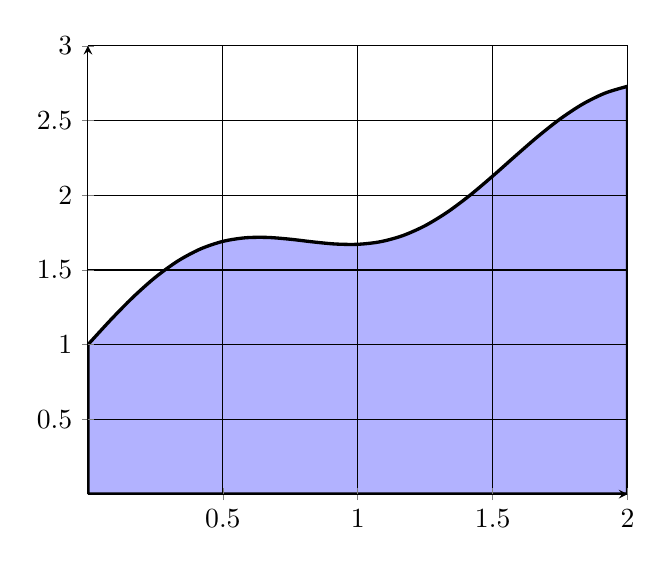
\begin{tikzpicture}
            \begin{axis}[axis lines=center, axis on top, grid,major grid style=black, xtick={0,0.5,1,1.5,2},
                ytick={0,0.5,1,1.5,2,2.5,3}, domain=0:2, ymin=0, ymax=3]
                \addplot[smooth, very thick, black, fill=blue!30] {0.25*sin(4*deg(x)) +
                    x*exp(-0.15*x)+1} \closedcycle;
            \end{axis}
        \end{tikzpicture}
    \end{center}
    \caption{Approximate the area under the curve between $x=0$ and $x=2$.}
    \label{fig:integral_ex1}
\end{figure}



In this section we will build methods for approximating integrals.  Recall from Calculus
that the definition of the Riemann integral is
\begin{flalign}
    \int_a^b f(x) dx = \lim_{\Delta x \to 0} \sum_{j=1}^N f(x_j) \Delta x
    \label{eqn:Riemann_integral}
\end{flalign}
where $N$ is the number of subintervals on the interval $[a,b]$ and $\Delta x$ is the
width of the interval.  As with differentiation, we can remove the limit and have a decent
approximation of the integral
\[ \int_a^b f(x) dx \approx \sum_{j=1}^N f(x_j) \Delta x. \]
You are likely familiar with this approximation of the integral from Calculus. The value of $x_j$ can
be chosen anywhere within the subinterval and three common choices are to use the left
endpoint, the midpoint, and the right endpoint.  We see
a depiction of this in Figure \ref{fig:integral_with_rectangles}.  

\begin{figure}[ht!]
    \begin{center}
        \begin{tikzpicture}[x=1.5cm, line cap=round, line join=round] 
            \foreach \k [count=\z] in {0, 1/4, 1/2}{
                \begin{scope}[shift=(0:\z*3)]
                    \path [plot fill, fill=red!30] plot [domain=0:2] (\x,{y(\x)}) -| cycle;
                    \foreach \x in {0, 1/2, 1, 3/2}
                    \path [bar, fill=blue!30]  (\x,0) |- (\x+1/2, {y(\x+\k)}) |- cycle;
                    \path [plot]  plot [domain=0:2] (\x,{y(\x)});
                    \path [axis] (0,4.5) |- (2.5,0);
                    \foreach \t [count=\x from 0] in {0,\frac{1}{2},1,\frac{3}{2},2}
                    \path [axis, -] (\x/2,0) -- ++(0,-3pt) node [below] {$\t$};
                    \foreach \y in {0,4}
                    \path [axis, -] (0,\y) -- ++(-3pt, 0) node [left] {$\y$};
                    \foreach \x in {0, 1/2, 1, 3/2}
                    \path [marking]  (\x+\k, {y(\x+\k)}) circle [radius=1.5pt];
                \end{scope}
            }
        \end{tikzpicture}
    \end{center}
    \caption{Riemann sum to approximate an integral with left, midpoint, and right
    rectangles on the function $f(x) = 4 - x^2$ on the interval $x \ in [0,2]$.}
    \label{fig:integral_with_rectangles}
\end{figure}

Clearly, the more rectangles we choose the closer the sum of the areas of the rectangles will get to the integral.
\begin{problem}
    Write \ProgLang code approximate an integral with Riemann sums. You should ALWAYS start by writing pseudo-code as comments in your
    \ProgLang file.    Your \ProgLang function
    should accept \ifnum\Python=0 an anonymous function handle\else a Python function\fi, a lower bound, an upper bound, the number
    of subintervals, and an optional input that allows the user to designate whether they
    want left, right, or midpoint rectangles. \\
    \ifnum\Python=0
    \mcode{function Area=MyRiemannSum(f, a, b, num_subintervals, type)}
    \else
    \mcode{def MyRiemannSum(f, a, b, num_subintervals, type):}
    \fi
    \\
    Test your code on several functions for which you know the integral.  You should write
    your code without any \mcode{for} loops.
\end{problem}

\begin{problem}\label{prob:left_riemann_error}
    Consider the function $f(x) = \sin(x)$.  We know the antiderivative for this function,
    $F(x) = -\cos(x) + C$, but in this question we are going to get a sense of the order
    of the error when doing Riemann Sum integration. 
    \begin{enumerate}
        \item[(a)] Find the exact value of 
            \[ \int_0^{1} f(x) dx. \]
        \item[(b)] Now build a Riemann Sum approximation (using your code) with various
            values of $\Delta x$.  For all of your approximation use left-justified
            rectangles.  Fill in the table with your results. 
            \begin{center}
                \begin{tabular}{|c|c|c|c|}
                    \hline
                    $\Delta x$ & Approx. Integral & Exact Integral & Abs. Percent Error \\
                    \hline \hline
                    $2^{-2} = 0.25$ & & & \\ \hline
                    $2^{-3} = 0.125$ & & & \\ \hline
                    $2^{-4}$ & & & \\ \hline
                    $2^{-5}$ & & & \\ \hline
                    $2^{-6}$ & & & \\\hline
                    $2^{-7}$ & & & \\\hline
                    $2^{-8}$ & & & \\\hline
                    $2^{-9}$ & & & \\ \hline
                \end{tabular}
            \end{center}
        \item[(c)] There was nothing really special about powers of 2 in part (b) of this
            problem.  Examine other sequences of $\Delta x$ with a goal toward answering
            the question: \\
            If we find an approximation of the integral with a fixed $\Delta x$ and find
            an absolute percent error, then what would happen to the absolute percent
            error if we divide $\Delta x$ by some positive constant $M$?
        \item[(d)] What is the apparent approximation error of the Riemann Sum method
            using left-justified rectangles.
    \end{enumerate}
\end{problem}

\begin{problem}
    Repeat Problem \ref{prob:left_riemann_error} using right-justified rectangles.  
\end{problem}


\begin{thm}
    In approximating the integral $\int_a^b f(x) dx$ with a fixed interval width $\Delta
    x$ we find an absolute percent error $P$.
    \begin{itemize}
    \item If we use left rectangles and an interval width of $\frac{\Delta x}{M}$ then the
        absolute percent error will be approximately \underline{\hspace{1in}}.
    \item If we use right rectangles and an interval width of $\frac{\Delta x}{M}$ then the
        absolute percent error will be approximately \underline{\hspace{1in}}.
    \end{itemize}
\end{thm}

The previous theorem could be stated in an equivalent way.

\begin{thm}
    In approximating the integral $\int_a^b f(x) dx$ with a fixed interval number of
    subintervals we find an absolute percent error $P$.
    \begin{itemize}
    \item If we use left rectangles and $M$ times as many subintervals then the
        absolute percent error will be approximately \underline{\hspace{1in}}.
    \item If we use right rectangles and $M$ times as many subintervals then the
        absolute percent error will be approximately \underline{\hspace{1in}}.
    \end{itemize}
\end{thm}

\begin{problem}
    Create a plot with the width of the subintervals on the horizontal axis and the
    absolute error between your (left) Riemann sum calculation and the exact integral for
    a known definite integral.  Your plot should be on a log-log scale.  Based on your
    plot, what is the approximate order of the error in the Riemann sum approximation?
\end{problem}

Now let's turn our attention to some slightly better algorithms for calculating the value
of a definite integral: The Trapezoidal Rule and Simpson's Rule.  There are many others,
but in practice these two are relatively easy to implement and have reasonably good error
approximations.  To motivate the idea of the Trapezoid rule consider Figure
\ref{fig:trap_motivation}.  It is plain to see that trapezoids will make better
approximations than rectangles at least in this particular case.  Another way to think
about using trapezoids, however, is to see the top side of the trapezoid as a secant line
connecting two points on the curve.  As $\Delta x$ gets arbitrarily small, the secant
lines become better and better approximations for tangent lines and are hence arbitrarily
good approximations for the curve.  For these reasons it seems like we should investigate
how to systematically approximate definite integrals via trapezoids.

\begin{figure}
    \begin{center}
        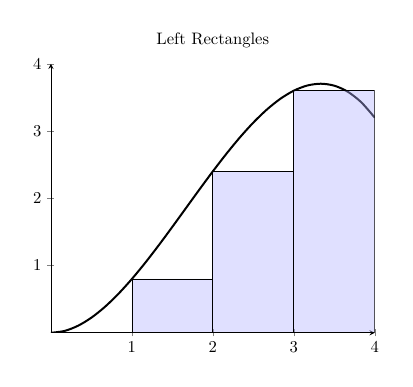
\begin{tikzpicture}[scale=0.6]
            \begin{axis}[axis lines=center, xmin=0, xmax=4, ymin=0, ymax=4, domain=0:4,
                title={Left Rectangles}]
                \addplot[smooth, very thick, black] {(1/5)*x^2*(5-x)};
                \draw[fill=blue!30, fill opacity=0.4] (axis cs:1,0) -- (axis cs:2,0) -- (axis cs:2,0.8) --
                (axis cs:1,0.8) -- (axis cs:1,0);
                \draw[fill=blue!30, fill opacity=0.4] (axis cs:2,0) -- (axis cs:3,0) --
                (axis cs:3,2.4) -- (axis cs:2,2.4) -- (axis cs:2,0);
                \draw[fill=blue!30, fill opacity=0.4] (axis cs:3,0) -- (axis cs:4,0) --
                (axis cs:4,3.6) -- (axis cs:3,3.6) -- (axis cs:3,0);
            \end{axis}
        \end{tikzpicture}
        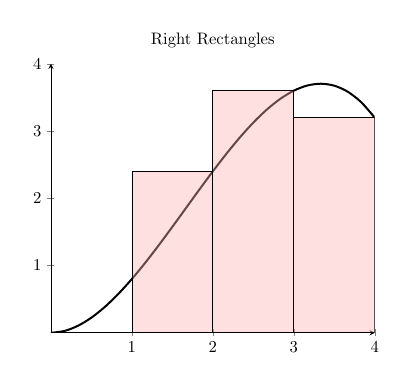
\begin{tikzpicture}[scale=0.6]
            \begin{axis}[axis lines=center, xmin=0, xmax=4, ymin=0, ymax=4, domain=0:4,
                title={Right Rectangles}]
                \addplot[smooth, very thick, black] {(1/5)*x^2*(5-x)};
                \draw[fill=red!30, fill opacity = 0.4] (axis cs:1,0) -- (axis cs:2,0) --
                (axis cs:2,2.4) -- (axis cs:1,2.4) -- (axis cs:1,0);
                \draw[fill=red!30, fill opacity = 0.4] (axis cs:2,0) -- (axis cs:3,0) --
                (axis cs:3,3.6) -- (axis cs:2,3.6) -- (axis cs:2,0);
                \draw[fill=red!30, fill opacity = 0.4] (axis cs:3,0) -- (axis cs:4,0) --
                (axis cs:4,3.2) -- (axis cs:3,3.2) -- (axis cs:3,0);
            \end{axis}
        \end{tikzpicture}
        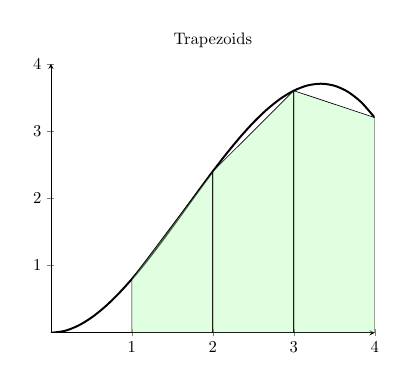
\begin{tikzpicture}[scale=0.6]
            \begin{axis}[axis lines=center, xmin=0, xmax=4, ymin=0, ymax=4, domain=0:4,
                title={Trapezoids}]
                \addplot[smooth, very thick, black] {(1/5)*x^2*(5-x)};
                \draw[fill=green!30, fill opacity = 0.4] (axis cs:1,0) -- (axis cs:2,0) --
                (axis cs:2,2.4) -- (axis cs:1,0.8) -- (axis cs:1,0);
                \draw[fill=green!30, fill opacity = 0.4] (axis cs:2,0) -- (axis cs:3,0) --
                (axis cs:3,3.6) -- (axis cs:2,2.4) -- (axis cs:2,0);
                \draw[fill=green!30, fill opacity = 0.4] (axis cs:3,0) -- (axis cs:4,0) --
                (axis cs:4,3.2) -- (axis cs:3,3.6) -- (axis cs:3,0);
            \end{axis}
        \end{tikzpicture}
    \end{center}
    \caption{Using rectangles and trapezoids with $\Delta x = 1$ for approximating
    the integral $\int_1^4 f(x)dx$.}
    \label{fig:trap_motivation}
\end{figure}

\begin{problem}
    Consider a single trapezoid approximating the area under a curve.  From geometry we
    recall that the area of a trapezoid is 
    \[ A = \frac{1}{2}\left( b_1 + b_2 \right) h \]
    where $b_1, b_2$ and $h$ are marked on the picture below.  The function shown in the
    picture is $f(x) = \frac{1}{5} x^2 (5-x)$.  Find the area of the shaded region as an
    approximation to
    \[ \int_1^4 \left( \frac{1}{5} x^2 (5-x) \right) dx. \]
    \begin{center}
        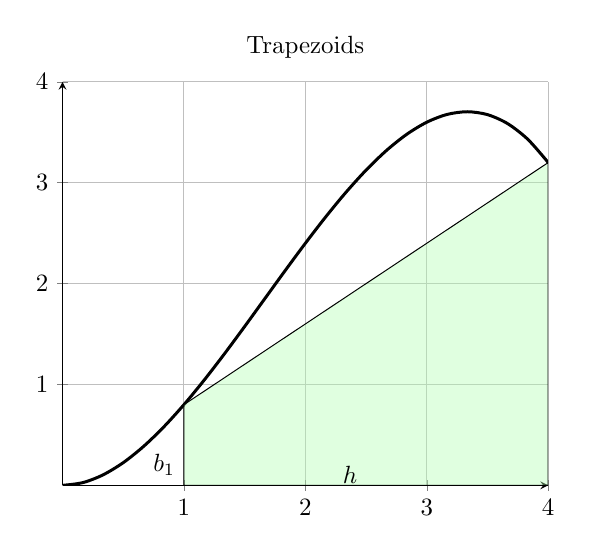
\begin{tikzpicture}[scale=0.9]
            \begin{axis}[axis lines=center, grid, xmin=0, xmax=4, ymin=0, ymax=4, domain=0:4,
                title={Trapezoids}]
                \addplot[smooth, very thick, black] {(1/5)*x^2*(5-x)};
                \draw[fill=green!30, fill opacity = 0.4] (axis cs:1,0) -- (axis cs:4,0) --
                (axis cs:4,3.2) -- (axis cs:1,0.8) -- (axis cs:1,0);
                \draw (axis cs:1,0.2) node[anchor=east]{$b_1$};
                \draw (axis cs:4,1.6) node[anchor=west]{$b_2$};
                \draw (axis cs:2.5,0.1) node[anchor=east]{$h$};
            \end{axis}
        \end{tikzpicture}
    \end{center}
\end{problem}

\begin{problem}
    Now use the same idea with $h = \Delta x = 1$ from figure \ref{fig:trap_motivation} to
    approximate the area under the function $f(x) = (1/5)x^2(5-x)$ between $x=1$ and $x=4$
    using three trapezoids.
\end{problem}

\begin{problem}
    Consider the function $f(x) = \frac{1}{5}x^2(5-x)$ again.
    \begin{enumerate}
        \item[(a)] Work out the exact value of the definite integral by hand.
        \item[(b)] Summarize your answers to the previous problems in the following table
            then extend the data that you have for smaller and smaller values of $\Delta
            x$.
            \begin{center}
                \begin{tabular}{|c|c|c|c|}
                    \hline
                    $\Delta x$ & Approx. Integral & Exact Integral & Abs. \% Error \\
                    \hline \hline
                    3 & & & \\ \hline
                    1 & & & \\ \hline
                    $1/3$ & & & \\ \hline
                    $1/9$ & & & \\ \hline
                    $\vdots$ & $\vdots$& $\vdots$& $\vdots$\\ \hline
                \end{tabular}
            \end{center}
        \item[(c)] From the table that you built in part (b), what do you conjecture is
            the order of the approximation error for the trapezoid method?
    \end{enumerate}
\end{problem}


\begin{technique}
    We want to approximate $\displaystyle \int_a^b f(x) dx$.  One of the simplest ways is
    to approximate the area under the function with a trapezoid.  Recall from basic
    geometry that area of a
    trapezoid is $A = \frac{1}{2} (b_1 + b_2) h$.  In terms of the integration problem we
    can do the following:
    \begin{enumerate}
        \item First partition $[a,b]$ into the set $\{x_0=a, x_1, x_2, \ldots, x_{n-1},
        x_n=b\}$.
        \item On each part of the partition approximate the area with a trapezoid:
            \[ A_j = \frac{1}{2} \left[ f(x_j) + f(x_{j-1}) \right]\left(
            x_j - x_{j-1} \right) \]
        \item Approximate the integral as
            \[ \int_a^b f(x) dx = \sum_{j=1}^n A_j \]
    \end{enumerate}
%     Draw a picture depicting how the trapezoidal rule works.
\end{technique}

\begin{problem}
    Write code to give the trapezoidal rule approximation for the definite integral
    $\int_a^b f(x) dx$.  Test your code on functions where you know the definite area.
    Then test your code on functions where you have approximated the area by examining a
    plot (i.e. you have a visual estimate of the area).
\end{problem}

\begin{problem}
    Use the code that you wrote in the previous problem to test your conjecture about the
    order of the approximation error for the trapezoid rule.  Integrate the function $f(x)
    = \sin(x)$ from $x=0$ to $x=1$ with more and more trapezoids.  In each case compare to
    the exact answer and find the absolute percent error.  The goal is to answer the
    question: \\
    {\it If I calculate the definite integral with a fixed $\Delta x$ and get an absolute
    percent error, $P$, then what absolute percent error will I get if I use a width of
$\Delta x / M$ for some positive number $M$?}
\end{problem}

The trapezoidal rule does a decent job approximating integrals, but ultimately you are
using linear functions to approximate $f(x)$ and the accuracy may suffer if the step
size is too large or the function too non-linear. You likely notice that the trapezoidal
rule will give an exact answer if you were to integrate a linear or constant function. A
potentially better approach would be to get an integral that evaluates quadratic functions
exactly. In order to do this we need to evaluate the function at three points (not two
like the trapezoidal rule). Let's integrate a function $f(x)$ on the interval
$[a,b]$ by using the three points $(a,f(a))$, $(m,f(m))$, and
$(b,f(b))$ where $m=\frac{a+b}{2}$ is the midpoint of the two boundary points. We want to
find constants $A1$, $A2$, and $A3$ such that the integral
\[ \int_a^b f(x) dx = A_1 f(a) + A_2 f\left( \frac{a+b}{2} \right) + A_3 f(b) \]
is exact for all constant, linear, and quadratic functions. This would guarantee that we
have an exact method for all polynomials of order 2 or less but should serve as a decent
approximation if the function is not quadratic.

To find the constants $A_1, A_2$, and $A_3$ we can write the following system of three
equations
\begin{flalign*}
    \int_a^b 1 dx &= b-a = A_1 + A_2 + A_3 \\
    \int_a^b x dx &= \frac{b^2 - a^2}{2} = A_1 a + A_2 \left( \frac{a+b}{2} \right) + A_3
    b \\
    \int_a^b x^2 dx &= \frac{b^3 - a^3}{3} = A_1 a^2 + A_2 \left( \frac{a+b}{2} \right)^2
    + A_3 b^2.
\end{flalign*}
Solving the linear system gives
\[ A_1 = \frac{b-a}{6}, \quad A_2 = \frac{4(b-a)}{6}, \quad \text{and} \quad
A_3 = \frac{b-a}{6}. \]
At this point we can see that the integral can be approximated as
\[ \int_a^b f(x) dx \approx \left( \frac{b-a}{6} \right) \left( f(a) + 4f\left(
    \frac{a+b}{2}
\right) + f(b) \right) \]
and the technique will give an exact answer for any polynomial of order 2 or below.  

\begin{problem}
    \begin{enumerate}
        \item[(a)] Use the method described above to approximate the area under the
            curve $f(x) = (1/5) x^2 (5-x)$ on the interval $[1,4]$.  To be clear, you will
            be using the points $a=1, m=2.5$, and $b=4$ in the above derivation.  
        \item[(b)] Next find the exact area under the curve $g(x) = (-1/2)x^2 +3.3x -2$ on
            the interval $[1,4]$.  
        \item[(c)] What do you notice about the two areas?  What does this sample problem
            tell you about the formula that we derived above?
    \end{enumerate}
    \begin{center}
        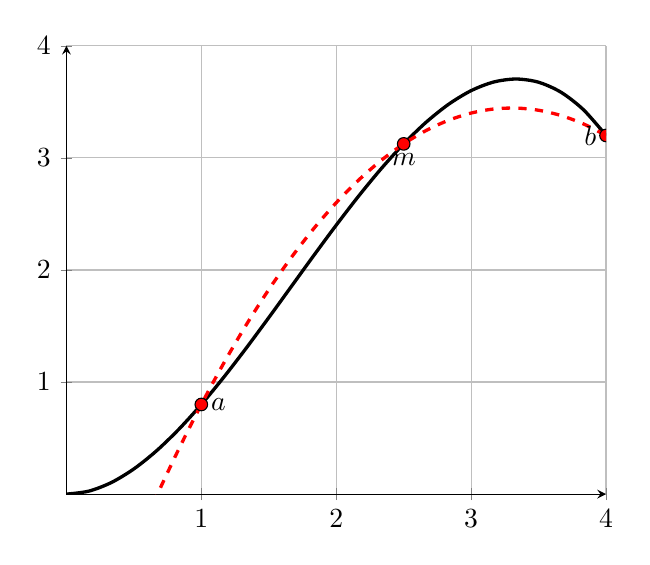
\begin{tikzpicture}
            \begin{axis}[axis lines=center, grid, xmin=0, xmax=4, ymin=0, ymax=4,
                domain=0:4]
                \addplot[smooth, black, very thick] {0.2*x^2*(5-x)};
                \addplot[smooth, red, dashed, very thick] {-0.5*x^2+3.3*x-2};
                \draw[fill=red] (axis cs:1,0.8) circle(0.08cm) node[anchor=west]{$a$};
                \draw[fill=red] (axis cs:2.5,3.125) circle(0.08cm) node[anchor=north]{$m$};
                \draw[fill=red] (axis cs:4,3.2) circle(0.08cm) node[anchor=east]{$b$};
            \end{axis}
        \end{tikzpicture}
    \end{center}
\end{problem}

To make the punchline of the previous problem a bit more clear, using the formula 
\[ \int_a^b f(x) dx \approx \left( \frac{a-b}{6} \right) \left( f(a) + 4 f(m) + f(b)
\right) \]
is the same as fitting a parabola to the three points $(a,f(a))$, $(m,f(m))$, and
$(b,f(b))$ and finding the area under the parabola exactly.  That is exactly the step up
from the trapezoid rule and Riemann sums that we were after: Riemann sums approxmiate the
function with constant functions, the trapezoid rule uses linear functions, and now we
have a method for approximating with parabolas.  

To improve upon this idea we now examine the problem of partitioning the interval $[a,b]$
into small pieces and running this process on each piece.  This is called Simpson's Rule
for integration.

\begin{technique}[Simpson's Rule]
    Now we put the process explained above into a form that can be coded to approximate
    integrals. We call this method Simpson's Rule after Thomas Simpson (1710-1761) who, by
    the way, was a basket weaver in his day job so he could pay the bills and keep doing
    math.
    \begin{enumerate}
        \item First parition $[a,b]$ into the set $\{x_0=a, x_1, x_2, \ldots, x_{n-1},
        x_n=b\}$.
        \item On each part of the partition approximate the area with a parabola:
            \[ A_j = \frac{1}{6} \left[ f(x_j) + 4 f\left( \frac{x_j+x_{j-1}}{2} \right) +
                f(x_{j-1}) \right]\left( x_j - x_{j-1} \right) \]
        \item Approximate the integral as
            \[ \int_a^b f(x) dx = \sum_{j=1}^n A_j \]
    \end{enumerate}
%     Draw a picture depicting how Simpson's rule works.
\end{technique}

\begin{problem}
    We have spent a lot of time over the past many pages building approximations of the
    order of the error for numerical integration and differentiation schemes.  It is now
    up to you.  \\
    Build a numerical experiment that allows you to conjecture the order of the
    approximation error for Simpson's rule.  Remember that the goal is to answer the
    question: \\
    If I approximate the integral with a fixed $\Delta x$ and find an absolute percent
    error of $P$, then what will the absolute percent error be using a width of $\Delta x
    / M$?
\end{problem}

\begin{problem}
    Write \ProgLang functions that implement both the trapezoidal rule and Simpson's rule.
    You should ALWAYS start by writing pseudo-code as comments in your \ProgLang file.   Keep
    in mind that \ProgLang \ifnum\Python=1(\texttt{numpy} arrays, specifically)\fi deals with vectors and iteration in very nice ways.  You shouldn't
    need a \texttt{for loop} in your function.

    Test both \ProgLang functions on known integrals and approximate the order of the error
    based on the mesh size.  
\end{problem}


Thus far we have three numerical approximations for definite integrals: Riemann sums (with
rectangles), the trapezoidal rule, and Simpsons's rule.  There are MANY other
approximations for integrals and we leave the further research to the curious reader.
\begin{thm}[Numerical Integration Techniques]\label{thm:num_int}
    Let $f(x)$ be a continuous function on the interval $[a,b]$.  The integral $\int_a^b
    f(x) dx$ can be approximated with any of the following.
    \begin{flalign*}
       &\text{Riemann Sum: }  \int_a^b f(x) dx \approx \sum_{j=1}^N f(x_j) \Delta x \\
       & \qquad \text{Error for Riemann Sums: } \mathcal{O}(\Delta x) \\
       &\text{Trapezoidal Rule: }  \int_a^b f(x) dx \approx \frac{1}{2} \sum_{j=1}^N
       \left( f(x_j) + f(x_{j-1}) \right) \Delta x \\
       & \qquad \text{Error for Trapezoidal Rule: } \mathcal{O}(\Delta x^2) \\
       &\text{Simpson's Rule: }  \int_a^b f(x) dx \approx \frac{1}{6} \sum_{j=1}^N \left(
       f(x_j) + 4 f\left( \frac{x_j + x_{j-1}}{2} \right) + f(x_{j-1}) \right) \Delta x \\
       & \qquad \text{Error for Simpson's Rule: } \mathcal{O}(\Delta x^4) \\
    \end{flalign*}
    where $\Delta x = x_j - x_{j-1}$ and $N$ is the number of subintervals.
\end{thm}

\begin{problem}
    Theorem \ref{thm:num_int} simply states the error rates for our three primary
    integration schemes.  For this problem you need to empirically verify these error
    rates.  Use the integration problem and exact answer
    \[ \int_0^{\pi/4} e^{3x} \sin(2x) dx = \frac{3}{13} e^{3\pi/4} + \frac{2}{13} \]
    and write code that produces a log-log error plot with $\Delta x$ on the horizontal axis and
    the absolute error on the vertical axis.  Fully explain how the error rates show
    themselves in your plot.
\end{problem}

\begin{example}
    In Figure \ref{fig:integration_errors} you'll see the error for our three primary integration techniques on the
    problem
    \[ \int_0^1 \sin(2x) dx \]
    which has an exact answer of 
    \[ \int_0^1 \sin(2x) dx = \frac{1}{2} - \frac{\cos(2)}{2}. \]  
    You'll see that Simpson's rule gains 4 orders of accuracy for every order of magnitude
    that the $\Delta x$ is decreased.  Similarly you'll see that
    Trapezoidal method gains 2 orders of magnitude of accuracy for every order of magnitude
    that $\Delta x$ is decreased, and Riemann sums only gain 1 order of magnitude.  Plots such
    as this can reveal the performance of a numerical method and give you a sense of how it is
    going to behave on a problem where you don't know the exact answer.
\end{example}

\begin{figure}[ht!]
    \begin{center}
        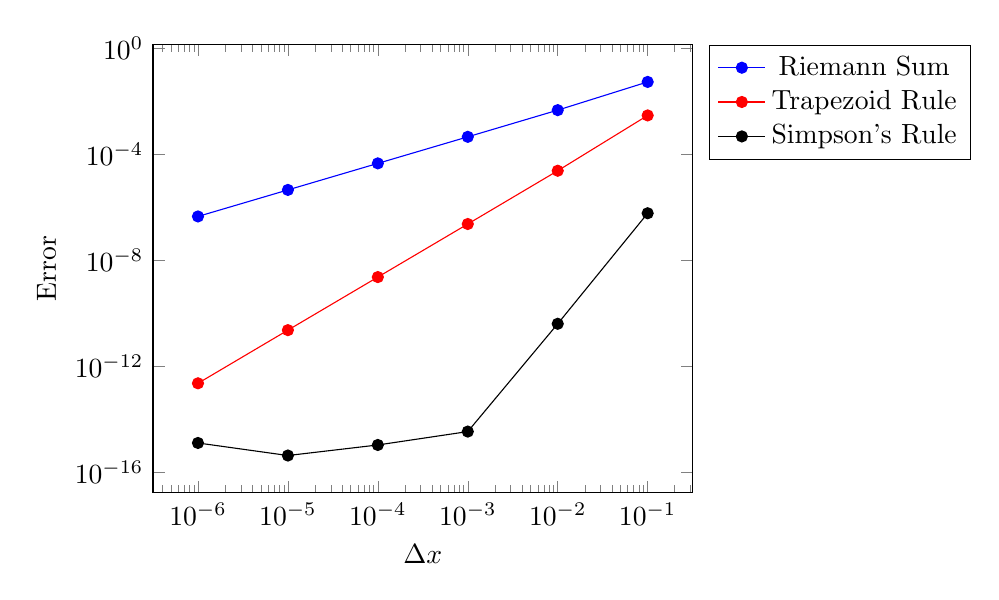
\begin{tikzpicture}
            \begin{loglogaxis}[xlabel={$\Delta x$}, ylabel={Error}, legend pos=outer north
                east]
                \addplot[color=blue, mark=*] coordinates {
               (0.10,0.0534328071726731)
               (0.0100,0.00461649308296008)
               (0.001000,0.000455340314476471)
               (0.00010000,0.0000454717790016046)
               (0.0000100000,0.00000454655620385491)
               (0.000001000000,0.00000045464940112705)
           };
           \addlegendentry{Riemann Sum}
                \addplot[color=red, mark=*] coordinates {
               (0.10,0.00291628346013517)
               (0.0100,0.000024)
               (0.001000,0.000000236)
               (0.00010000,0.00000000236)
               (0.0000100000,0.0000000000236)
               (0.000001000000,0.000000000000234)
           };
           \addlegendentry{Trapezoid Rule}
                \addplot[color=black, mark=*] coordinates {
               (0.10,0.0000006)
               (0.0100,0.000000000041)
               (0.001000,0.00000000000000355)
               (0.00010000,0.00000000000000111)
               (0.0000100000,0.000000000000000444)
               (0.000001000000,0.00000000000000132)
           };
           \addlegendentry{Simpson's Rule}
            \end{loglogaxis}
        \end{tikzpicture}
    \end{center}
    \caption{Errors with integration techniques.}
    \label{fig:integration_errors}
\end{figure}






\newpage\section{Optimization}
You likely recall that one of the major applications of Calculus was to solve optimization
problems -- find the value of $x$ which makes some function as big or as small as
possible.  The process itself can sometimes be rather challenging due to either the
modeling aspect of the problems and/or the fact that the differentiation might be
quite cumbersome.  In this section we will revisit those problems from Calculus, but our
goal will be to build a numerical method for the Calculus step in hopes to avoid the messy
algebra and differentiation.

\begin{problem}[The Classic Cardboard Box Problem]\label{prob:cardboard}
    A piece of cardboard measuring 20cm by 20cm is to be cut so that it can be folded into
    a box without a lid. We want to find the size of the cut, $x$, that maximizes the
    volume of the box. 
    \begin{center}
        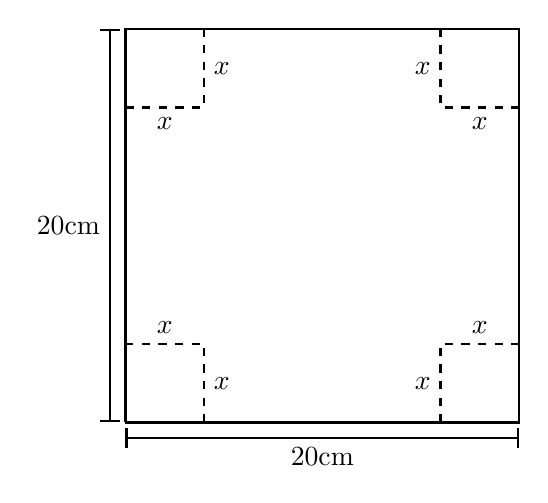
\begin{tikzpicture}
            \draw[thick, black] (0,0) -- (5,0) -- (5,5) -- (0,5) -- (0,0);
            \draw[dashed, thick] (1,0) -- (1,1) -- (0,1);
            \draw[dashed, thick] (4,0) -- (4,1) -- (5,1);
            \draw[dashed, thick] (4,5) -- (4,4) -- (5,4);
            \draw[dashed, thick] (0,4) -- (1,4) -- (1,5);
            \draw[thick, |-|] (0,-0.2) -- (5,-0.2);
            \draw (2.5,-0.2) node[anchor=north]{$20$cm};
            \draw[thick, |-|] (-0.2,0) -- (-0.2,5);
            \draw (-0.2,2.5) node[anchor=east]{$20$cm};
            \draw (1,0.5) node[anchor=west]{$x$};
            \draw (4,0.5) node[anchor=east]{$x$};
            \draw (4,4.5) node[anchor=east]{$x$};
            \draw (1,4.5) node[anchor=west]{$x$};
            \draw (0.5,1) node[anchor=south]{$x$};
            \draw (4.5,1) node[anchor=south]{$x$};
            \draw (0.5,4) node[anchor=north]{$x$};
            \draw (4.5,4) node[anchor=north]{$x$};
        \end{tikzpicture}
    \end{center}
    \begin{enumerate}
        \item[(a)] Write a function for the volume of the box resulting from a cut of size
            $x$.  What is the domain of your function?
        \item[(b)] We know that we want to maximize this function so go through the
            full Calculus exercise to find the maximum:
            \begin{itemize}
                \item take the derivative
                \item set it to zero
                \item find the critical points
                \item test the critical points and the boundaries of the domain using the
                    extreme value theorem to determine the $x$ that gives the maximum.
            \end{itemize}
    \end{enumerate}
\end{problem}

% \newpage\subsection{Single Variable Numerical Optimization}

Now we'll propose a few numerical techniques that can approximate the solution to these
types of problems.  The basic ideas are simple!

\begin{problem}\label{prob:intuitive_max}
    If you were blind folded and standing on a hill could you find the top of the hill?
    (assume no trees and no cliffs \ldots this isn't supposed to be dangerous)  How would
    you do it?  Explain your technique clearly.
\end{problem}

\begin{problem}
    If you were blind folded and standing on a crater on the moon could you find the
    lowest point?  How would you do it?  Remember that you can hop as far as you like
    \ldots because gravity \ldots but sometimes that's not a great thing because you could
    hop too far.
\end{problem}

The intuition of numerical optimization schemes is typically to visualize the function that
you're trying to minimize or maximize and think about either climbing the hill to the top
(maximization) or descending the hill to the bottom (minimization).  

\begin{problem}
    Let's turn your intuition into an algorithm.  If $f(x)$ is the function that you are
    trying to maximize then turn your algorithm from Problem \ref{prob:intuitive_max} into
    a step-by-step algorithm which could be coded. Then try out your code on the function 
    \[ f(x) = e^{-x^2} + \sin(x^2) \]
    to see if your algorithm can find the local maximum near $x \approx 1.14$.
\end{problem}

Some of the most common algorithms are listed below.  Read through them and see which
one(s) you ended up recreating?  The intuition for these algorithms is pretty darn simple
-- travel uphill if you want to maximize -- travel downhill if you want to minimize.

\begin{algorithm}[Derivative Free Optimization]
    Let $f(x)$ be the objective function which you are seeking to maximize (or minimize).
    \begin{itemize}
        \item Pick a starting point, $x_0$, and find the value of your
            objective function at this point, $f(x_0)$.
        \item Pick a small step size (say, $\Delta x \approx 0.01$).
        \item Calculate the objective function one step to the left and
            one step to the right from your starting point.  Which ever
            point is larger (if you're seeking a maximum) is the point
            that you keep for your next step.
        \item Iterate (decide on a good stopping rule)
    \end{itemize}
\end{algorithm}
\begin{problem}
    Write code to implement the 1D derivative free optimization algorithm and use it to solve
    Problem \ref{prob:cardboard}.  Compare your answer to the analytic solution.
\end{problem}

\begin{algorithm}[Gradient Ascent/Descent]
    Let $f(x)$ be the objective function which you are seeking to maximize (or minimize).
    \begin{itemize}
        \item Find the derivative of your objective function, $f'(x)$.
        \item Pick a starting point, $x_0$.
        \item Pick a small control parameter, $\alpha$ (in machine learning this parameter
            is called the ``learning rate'' for the gradient descent algorithm).
        \item Use the iteration $x_{n+1} = x_n + \alpha f'(x_n) $ if you're maximizing.
            Use the iteration $x_{n+1} = x_n - \alpha f'(x_n)$ if you're minimizing.
        \item Iterate (decide on a good stopping rule)
    \end{itemize}
\end{algorithm}
% \begin{problem}
%     Give graphical reasoning for the formula given in the 1D gradient descent algorithm.
%     Also decide what will happen in the algorithm if $\alpha$ is larger or smaller.
% \end{problem}

\begin{problem}
    Write code to implement the 1D gradient descent algorithm and use it to solve
    Problem \ref{prob:cardboard}. Compare your answer to the analytic solution.
\end{problem}

\begin{algorithm}[Monte Carlo Search]
    Let $f(x)$ be the objective function which you are seeking to maximize (or minimize).
    \begin{itemize}
        \item Pick many (perhaps several thousand!) different $x$ values.
        \item Find the value of the objective function at every one of
            these points (Hint: use lists, not loops)
        \item Keep the $x$ value that has the largest (or smallest if
            you're minimizing) value of the objective function.
        \item Iterate many times and compare the function value in each
            iteration to the previous best function value
    \end{itemize}
\end{algorithm}
\begin{problem}
    Write code to implement the 1D monte carlo search algorithm and use it to solve
    Problem \ref{prob:cardboard}. Compare your answer to the analytic solution.
\end{problem}

\begin{algorithm}[Optimization via Numerical Root Finding]
    Let $f(x)$ be the objective function which you are seeking to maximize (or minimize).
    \begin{itemize}
        \item Find the derivative of your objective function.
        \item Set the derivative to zero and use a numerical root finding
            method (such as bisection or Newton) to find the critical
            point.
        \item Use the extreme value theorem to determine if the critical point or one of
            the endpoints is the maximum (or minimum).
    \end{itemize}
\end{algorithm}
\begin{problem}
    Write code to implement the 1D numerical root finding optimization algorithm and use
    it to solve Problem \ref{prob:cardboard}. Compare your answer to the analytic solution.
\end{problem}





\begin{problem}
    In this problem we will compare an contrast the four methods proposed in the previous
    problem.
    \begin{enumerate}
        \item[(a)] What are the advantages to each of the methods proposed?
        \item[(b)] What are the disadvantages to each of the methods proposed?
        \item[(c)] Which method, do you suppose, will be faster in general?  Why?
        \item[(d)] Which method, do you suppose, will be slower in general?  Why?
    \end{enumerate}
\end{problem}

\begin{problem}
    The Gradient Ascent/Descent algorithm is the most geometrically interesting of the
    four that we have proposed.  The others are pretty brute force algorithms.  What is
    the Gradient Ascent/Descent algorithm doing geometrically?  Draw a picture and be
    prepared to explain to your peers.
\end{problem}


\begin{problem}\label{prob:pig_numerical}
    (This problem is modified from \cite{Meerschaert}) \\
    A pig weighs 200 pounds and gains weight at a rate proportional to its current weight.
    Today the growth rate if 5 pounds per day.  The pig costs 45 cents per day to keep due
    mostly to the price of food.  The market price for pigs if 65 cents per pound but is
    falling at a rate of 1 cent per day.  When should the pig be sold and how much profit
    do you make on the pig when you sell it?  Write this situation as a single variable
    mathematical model and solve the problem analytically (by hand).  Then solve the
    problem with all four methods outlined thus far in this section.
\end{problem}

\begin{problem}
    (This problem is modified from \cite{Meerschaert}) \\
    Reconsider the pig problem \ref{prob:pig_numerical} but now suppose that the weight of
    the pig after $t$ days is 
    \[ w = \frac{800}{1+3e^{-t/30}} \text{ pounds}. \]
    When should the pig be sold and how much profit do you make on the pig when you sell
    it?  Write this situation as a single variable mathematical model.  You should notice
    that the algebra and calculus for solving this problem is no longer really a desirable
    way to go.  Use an appropriate numerical technique to solve this problem.
\end{problem}



\begin{problem}
    Numerical optimization is often seen as quite challenging since the algorithms that
    we have introduced here could all get ``stuck'' at local extrema.  To illustrate this
    see the function shown in Figure \ref{fig:num_opt_challenging}.  How will derivative
    free optimization methods have trouble finding the red point starting at the black
    point with this function?  How will gradient
    descent/ascent methods have trouble?  Why?
\end{problem}

\begin{figure}
    \begin{center}
        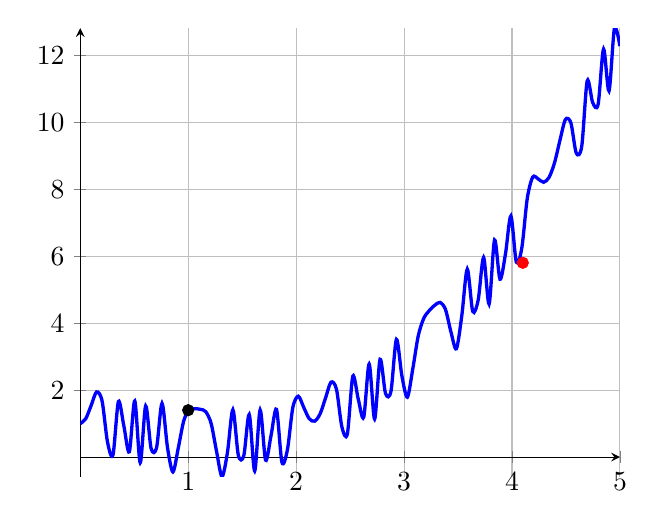
\begin{tikzpicture}
            \begin{axis}[axis lines=center, grid]
                \addplot[smooth, blue, very thick, domain=0:5, samples=100] {exp(-x^2) +
                sin(deg(x)^2) + 0.1*x^3};
                \addplot[black, only marks, mark=*] coordinates{(1,1.4)};
                \addplot[red, only marks, mark=*] coordinates{(4.1,5.8)};
            \end{axis}
        \end{tikzpicture}
    \end{center}
    \caption{A challenging numerical optimization problem. If we start at the black point
    then how will any of our algorithms find the local minimum at the red point?}
    \label{fig:num_opt_challenging}
\end{figure}



\newpage\section{Curve Fitting -- The Least Squares Problem via Numerical Optimization}
In this section we'll change our focus a bit to look at a different question from algebra,
and, in turn, reveal a hidden numerical optimization problem.
Instead of finding the roots of an algebraic equation, what if we have a few data points
and a reasonable guess for the type of function fitting the points, how would we determine
the actual function?  

\begin{problem}
    Consider the function $f(x)$ that goes exactly through the points $(0,1)$, $(1,4)$,
    and $(2,13)$.  
    \begin{enumerate}
        \item[(a)] Find a function that goes through these points exactly.  Be able to
            defend your work.
        \item[(b)] Is your function unique?  That is to say, is there another function out
            there that also goes exactly through these points?  
    \end{enumerate}
\end{problem}

\begin{problem}
    Now let's make a minor tweak to the previous problem.  Let's say that we have the data
    points $(0,1.07)$, $(1,3.9)$, $(2,14.8)$, and $(3,26.8)$.  Notice that these points
    are {\it close} to the points we had in the previous problem, but all of the $y$
    values have a little noise in them and we have added a fourth point.  If we suspect
    that a function $f(x)$ that {\it best} fits this data is quadratic then $f(x) = ax^2 +
    bx + c$ for some constants $a$, $b$, and $c$.  
    \begin{enumerate}
        \item[(a)] Plot the four points along with the function $f(x)$ for arbitrarily
            chosen values of $a$, $b$, and $c$.  
        \item[(b)] Work with your partner(s) to systematically change $a$, $b$, and $c$ so
            that you get a good visual match to the data.  
        \item[(c)] Now let's be a bit more systematic about things.  Let's say that you
            have a pretty good guess that $b \approx 2$ and $c \approx 0.7$.  We need to
            get a good estimate for $a$.
            \begin{enumerate}
                \item[(i)] Pick an arbitrary starting value for $a$.  For each
                    of the four points find the error between the predicted $y$ value and
                    the actual $y$ value.
                \item[(ii)] Square all four of your errors and add them up.  (Stop and
                    think: why are we squaring the errors before we sum them \ldots have a
                    discussion here)
                \item[(iii)] Now change your value of $a$ to several different values and
                    record the sum of the square errors for each of your values of $a$. It
                    may be worth while to use a spreadsheet to keep track of your work
                    here.
                \item[(iv)] Make a plot with the value of $a$ on the horizontal axis and
                    the value of the sum of the square errors on the vertical axis.  Use
                    your plot to defend the optimal choice for $a$.
            \end{enumerate}
    \end{enumerate}
\end{problem}

\begin{problem}
    We're going to revisit part (c) of the previous problem.  Write a loop that tries many
    values of $a$ in very small increments and calculates the sum of the squared errors.
    Have your loop stop when you think that it has reached the best value of $a$.
\end{problem}


\begin{technique}[Nonlinear Least Squares Curve Fitting]\label{tech:least_squares}
    Let 
    \[ S = \{ (x_1, y_1), \, (x_2, y_2), \, \ldots, \, (x_n, y_n) \} \] 
    be a set of $n$
    ordered pairs in $\mathbb{R}^2$.  If we guess that a function $f(x)$ is a best choice
    to fit the data and if $f(x)$ depends on parameters $a_1, a_2, \ldots$ then 
    \begin{enumerate}
        \item Pick initial values for the parameters $a_1, a_2, \ldots$ so that the
            function $f(x)$ {\it looks like} it is close to the data (this is strictly a
            visual step \ldots take care that it may take some playing around to guess the
            initial values of the parameters)
        \item Calculate the square error between the data point and the prediction from the
            function $f(x)$
            \[ \text{error for the point $x_i$: } e_i = \left( y_i - f(x_i) \right)^2. \]
            Note that squaring the error has the advantages of removing the sign,
            accentuating errors larger than 1, and decreasing errors that are less than 1.
        \item As a measure of the total error between the function and the data, sum the
            squared errors 
            \[ \text{sum of square errors } = \sum_{i=1}^n \left( y_i - f(x_i) \right)^2.
            \]
            (Take note that if there were a continuum of points instead of a discrete set
            then we would integrate the square errors instead of taking a sum.)
        \item Change the parameters $a_1, a_2, \ldots$ so as to minimize the sum of the
            square errors.
    \end{enumerate}
\end{technique}

In Technique \ref{tech:least_squares} the last step is a bit vague.  That was purposeful
since there are many techniques that could be used to minimize the sum of the square
errors.  In this particular section of this text we'll look at two of them: (1) Solver in
MS Excel and (2) 
\ifnum\Python=0 \texttt{fminsearch} in MATLAB.
\else
\texttt{scipy.optimize.fmin} in Python's \texttt{scipy} package.
\fi
Before we get into how those techniques
work let's look at an example of how the minimization step works graphically.

Let's return to the data set 
\[ S = \{ (0,1.07), \, (1,3.9), \, (2,14.8), \, (3,26.8)\} \]
under the assumption that the curve we want to use is quadratic: $f(x) = ax^2 + bx +
c$.\footnote{Take note that since we have four points then we could find an exact
    interpolating fit if we used a cubic function instead, but that isn't the point.  In
    fact, using higher order polynomials has the disadvantage of potentially fitting the
curve to measurement noise.} In Figure \ref{fig:least_squares_ex} we see the points in red
along with several guesses for the values of the parameters.  In these figures we are just
changing one of the parameters while keeping the other two fixed for easier illustration.
In reality we should note that all three of the parameters need to be changed to achieve
the desired minimization.  

\begin{figure}
    \begin{center}
        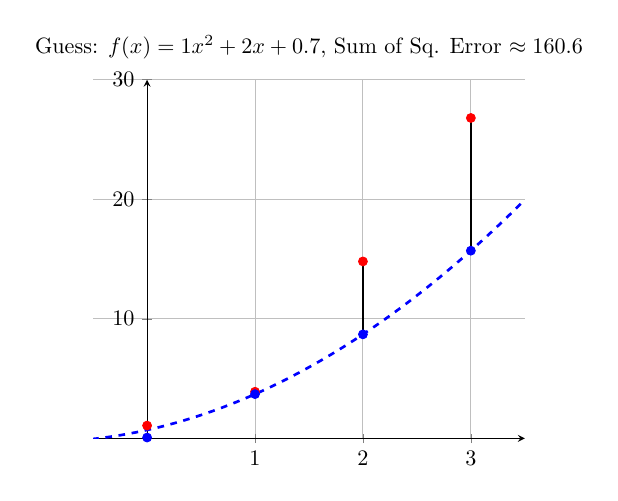
\begin{tikzpicture}[scale=0.8]
            \begin{axis}[axis lines=center, grid, xmin=-0.5, xmax=3.5, ymin=0, ymax=30,
                domain=-1:3.5, title={Guess: $f(x) = 1x^2 + 2x + 0.7$, Sum of Sq. Error
                $\approx 160.6$}]
                \addplot[smooth, very thick, blue, dashed] {1.0*x^2 + 2*x + 0.7};
                \addplot[only marks, mark=*, red]
                coordinates{(0,1.07)(1,3.9)(2,14.8)(3,26.8)};
                \addplot[only marks, mark=*, blue]
                coordinates{(0,0.07)(1,3.7)(2,8.7)(3,15.7)};
                \draw[very thick, black] (axis cs:0,1.07) -- (axis cs:0,0.7);
                \draw[very thick, black] (axis cs:1,3.90) -- (axis cs:1,3.7);
                \draw[very thick, black] (axis cs:2,14.8) -- (axis cs:2,8.7);
                \draw[very thick, black] (axis cs:3,26.8) -- (axis cs:3,15.7);
            \end{axis}
        \end{tikzpicture}
        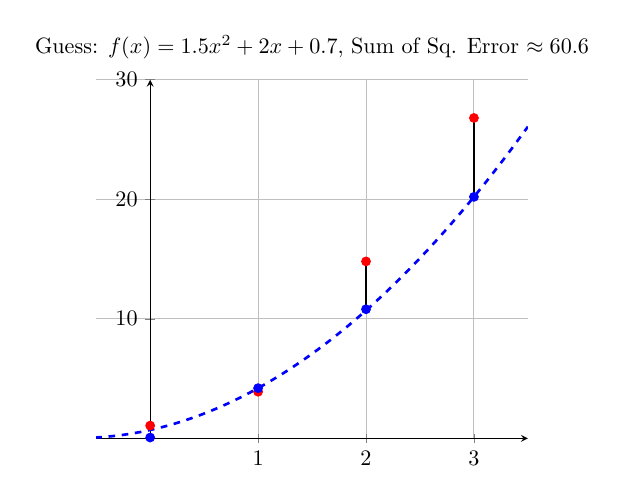
\begin{tikzpicture}[scale=0.8]
            \begin{axis}[axis lines=center, grid, xmin=-0.5, xmax=3.5, ymin=0, ymax=30,
                domain=-1:3.5, title={Guess: $f(x) = 1.5x^2 + 2x + 0.7$, Sum of Sq. Error
                $\approx 60.6$}]
                \addplot[smooth, very thick, blue, dashed] {1.5*x^2 + 2*x + 0.7};
                \addplot[only marks, mark=*, red]
                coordinates{(0,1.07)(1,3.9)(2,14.8)(3,26.8)};
                \addplot[only marks, mark=*, blue]
                coordinates{(0,0.07)(1,4.2)(2,10.8)(3,20.2)};
                \draw[very thick, black] (axis cs:0,1.07) -- (axis cs:0,0.7);
                \draw[very thick, black] (axis cs:1,3.90) -- (axis cs:1,4.2);
                \draw[very thick, black] (axis cs:2,14.8) -- (axis cs:2,10.8);
                \draw[very thick, black] (axis cs:3,26.8) -- (axis cs:3,20.2);
            \end{axis}
        \end{tikzpicture}
        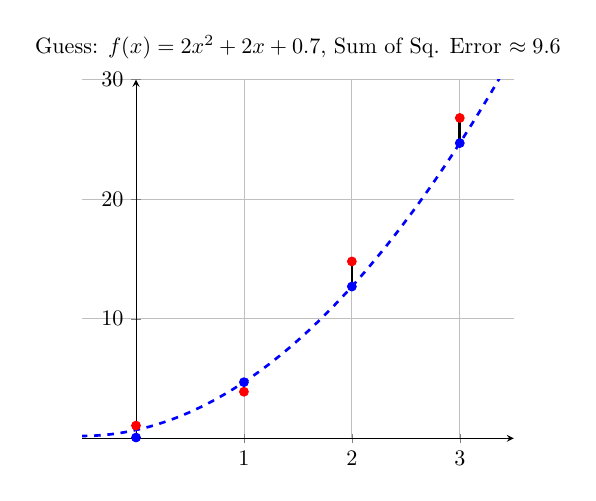
\begin{tikzpicture}[scale=0.8]
            \begin{axis}[axis lines=center, grid, xmin=-0.5, xmax=3.5, ymin=0, ymax=30,
                domain=-1:3.5, title={Guess: $f(x) = 2x^2 + 2x + 0.7$, Sum of Sq. Error
                $\approx 9.6$}]
                \addplot[smooth, very thick, blue, dashed] {2*x^2 + 2*x + 0.7};
                \addplot[only marks, mark=*, red]
                coordinates{(0,1.07)(1,3.9)(2,14.8)(3,26.8)};
                \addplot[only marks, mark=*, blue]
                coordinates{(0,0.07)(1,4.7)(2,12.7)(3,24.7)};
                \draw[very thick, black] (axis cs:0,1.07) -- (axis cs:0,0.7);
                \draw[very thick, black] (axis cs:1,3.90) -- (axis cs:1,4.7);
                \draw[very thick, black] (axis cs:2,14.8) -- (axis cs:2,12.7);
                \draw[very thick, black] (axis cs:3,26.8) -- (axis cs:3,24.7);
            \end{axis}
        \end{tikzpicture}
        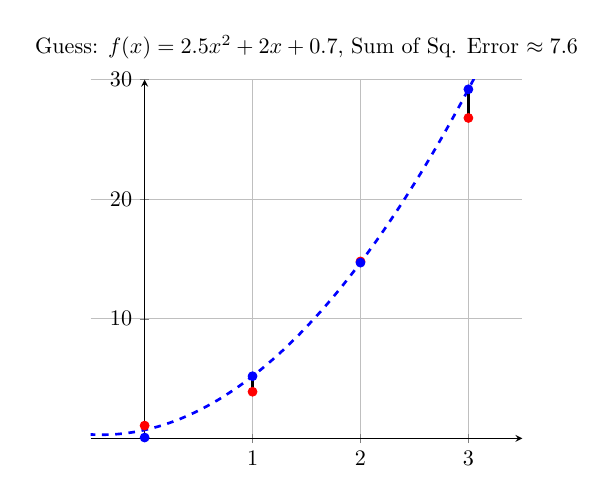
\begin{tikzpicture}[scale=0.8]
            \begin{axis}[axis lines=center, grid, xmin=-0.5, xmax=3.5, ymin=0, ymax=30,
                domain=-1:3.5, title={Guess: $f(x) = 2.5x^2 + 2x + 0.7$, Sum of Sq. Error
                $\approx 7.6$}]
                \addplot[smooth, very thick, blue, dashed] {2.5*x^2 + 2*x + 0.7};
                \addplot[only marks, mark=*, red]
                coordinates{(0,1.07)(1,3.9)(2,14.8)(3,26.8)};
                \addplot[only marks, mark=*, blue]
                coordinates{(0,0.07)(1,5.2)(2,14.7)(3,29.2)};
                \draw[very thick, black] (axis cs:0,1.07) -- (axis cs:0,0.7);
                \draw[very thick, black] (axis cs:1,3.90) -- (axis cs:1,5.2);
                \draw[very thick, black] (axis cs:2,14.8) -- (axis cs:2,14.7);
                \draw[very thick, black] (axis cs:3,26.8) -- (axis cs:3,29.2);
            \end{axis}
        \end{tikzpicture}
    \end{center}
    \caption{Demonstration of the curve fitting technique. The vertical black bars between
    the points show the point-wise error in the estimate. In these four pictures we are
only modifying the value of $a$ while leaving $b = 2$ and $c=0.7$ fixed for simplicity.
In reality we need to change all three parameters in the minimization process - hence the
actual minimization takes place in three dimensions.}
    \label{fig:least_squares_ex}
\end{figure}

In Figure \ref{fig:least_squares_ex} we saw that for $b=2$ and $c=0.7$ then the quadratic
function $f(x) \approx 2.5 x^2 + 2x + 0.7$ is a pretty good approximation of the data $S =
\{ (0,1.07), \, (1,3.9), \, (2,14.8), \, (3,26.8)\}.$ If, however, we take finer
increments between our guesses for $a$ we can get a refined estimate of the value of $a$
that minimizes the sum of the squared errors.  In Figure
\ref{fig:least_squares_ex_error_plot} we see the values of the sum of the squared errors
for many estimates of $a$.  In \ref{fig:least_squares_ex_error_plot} we see that $a
\approx 2.3$ gives a slightly better value of the sum of the square errors and is
(visually) near the minimum of the error curve.  

\begin{figure}
    \begin{center}
        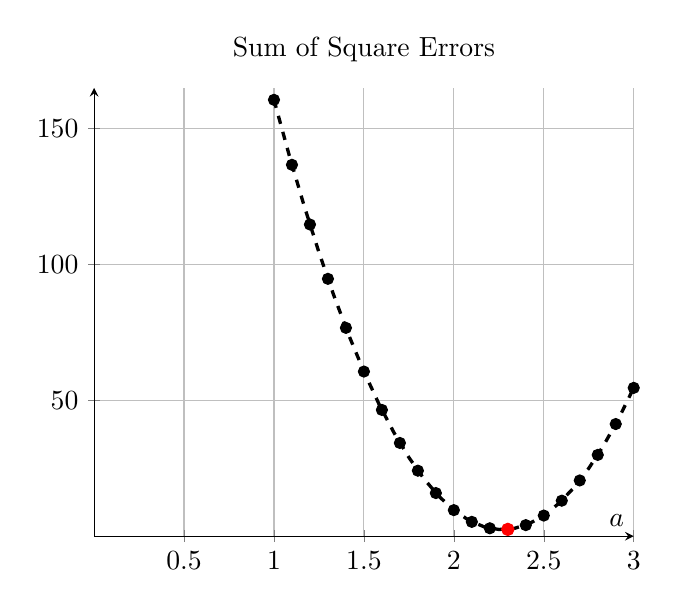
\begin{tikzpicture}
            \begin{axis}[axis lines=center, grid, xmin=0, xmax=3, ymin=0, ymax=165,
                xlabel={$a$}, title={Sum of Square Errors}]
                \addplot[very thick, black, dashed, domain=1:3] {98*x^2 - 445*x + 507.6};
                \addplot[black, only marks, mark=*] coordinates{
(1,160.5969)
(1.1,136.6769)
(1.2,114.7169)
(1.3,94.7169)
(1.4,76.6769)
(1.5,60.5969)
(1.6,46.4769)
(1.7,34.3169)
(1.8,24.1169)
(1.9,15.8769)
(2,9.5969)
(2.1,5.2769)
(2.2,2.9169)
(2.3,2.5169)
(2.4,4.0769)
(2.5,7.5969)
(2.6,13.0769)
(2.7,20.5169)
(2.8,29.9169)
(2.9,41.2769)
(3,54.5969)};
                \addplot[only marks, thick, red, mark=*] coordinates{(2.3,2.51)};
            \end{axis}
        \end{tikzpicture}
    \end{center}
    \caption{The sum of the squared errors for the function $f(x) = ax^2 + bx + c$ for the
    data set $S = \{ (0,1.07), \, (1,3.9), \, (2,14.8), \, (3,26.8)\}$. For $b=2$ and
$c=0.7$ the minimum occurs on this curve at approximately $a \approx 2.3$ with the sum of
the square errors of approximately 2.51. (To build this plot we took increments of $0.1$
between different guesses for $a$ from $1$ to $3$ -- a very brute-force way of
approximating a minimum.}
    \label{fig:least_squares_ex_error_plot}
\end{figure}


\begin{problem}\label{prob:least_squares_plots}
    For each of the plots in Figure \ref{fig:plot_least_squares_prob} give a functional
    form that {\it might} be a good model for the data.  Be sure to choose the most
    general form of your guess (for example, if you choose ``quadratic'' then your
    functional guess is $f(x) = ax^2 + bx + c$).  Once you have a guess of the function
    type create a plot showing your data along with your guess for a reasonable set of
    parameters. Your instructor will make the data available to you.
\end{problem}


\begin{figure}
    \begin{center}
        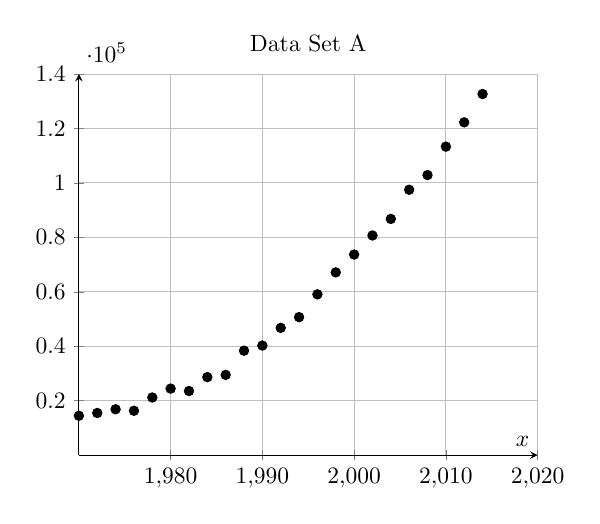
\begin{tikzpicture}[scale=0.85]
            \begin{axis}[axis lines=center, grid, xmin=1970, xmax=2020, ymin=0,
                ymax=140000, ytick={20000,40000,60000,80000,100000,120000,140000},
            xtick={1970, 1980, 1990, 2000, 2010, 2020}, xlabel={$x$}, title={Data Set A}]
                \addplot[only marks, mark=*, black] coordinates{
(1970,14443)
(1972,15465)
(1974,16831)
(1976,16280)
(1978,21159)
(1980,24427)
(1982,23541)
(1984,28643)
(1986,29463)
(1988,38355)
(1990,40244)
(1992,46740)
(1994,50676)
(1996,59060)
(1998,67122)
(2000,73668)
(2002,80678)
(2004,86763)
(2006,97481)
(2008,102878)
(2010,113314)
(2012,122238)
(2014,132645)};
            \end{axis}
        \end{tikzpicture}
        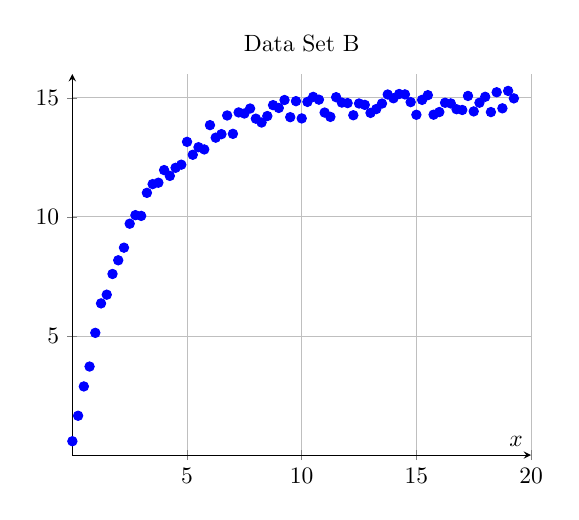
\begin{tikzpicture}[scale=0.85]
            \begin{axis}[axis lines=center, xmin=0, xmax=20, ymin=0, ymax=16, grid,
                xlabel={$x$}, title={Data Set B}]
                \addplot[only marks, mark=*, blue] coordinates{
(0,0.582100861)
(0.25,1.651055541)
(0.5,2.882416411)
(0.75,3.717797895)
(1,5.132399665)
(1.25,6.369000119)
(1.5,6.734741617)
(1.75,7.604108155)
(2,8.178632241)
(2.25,8.708613982)
(2.5,9.714736882)
(2.75,10.07421665)
(3,10.04271604)
(3.25,11.01046563)
(3.5,11.37732629)
(3.75,11.43607843)
(4,11.96616171)
(4.25,11.72225998)
(4.5,12.0620352)
(4.75,12.19243965)
(5,13.15165084)
(5.25,12.60932538)
(5.5,12.92675124)
(5.75,12.83330417)
(6,13.85374617)
(6.25,13.32748754)
(6.5,13.47426035)
(6.75,14.25917749)
(7,13.48781964)
(7.25,14.38714334)
(7.5,14.34069055)
(7.75,14.55105169)
(8,14.12389207)
(8.25,13.96255959)
(8.5,14.23544928)
(8.75,14.69309385)
(9,14.57472964)
(9.25,14.90832914)
(9.5,14.18763374)
(9.75,14.8603983)
(10,14.13555604)
(10.25,14.83016945)
(10.5,15.03918587)
(10.75,14.9228424)
(11,14.38124871)
(11.25,14.20006999)
(11.5,15.02628609)
(11.75,14.80054635)
(12,14.77921618)
(12.25,14.26918288)
(12.5,14.76285923)
(12.75,14.70457635)
(13,14.36665995)
(13.25,14.52763132)
(13.5,14.7602034)
(13.75,15.13930503)
(14,14.98096155)
(14.25,15.16100739)
(14.5,15.14435175)
(14.75,14.8201741)
(15,14.28843305)
(15.25,14.91406464)
(15.5,15.1121328)
(15.75,14.2922203)
(16,14.40273029)
(16.25,14.79309362)
(16.5,14.76448318)
(16.75,14.522059)
(17,14.48959447)
(17.25,15.07954907)
(17.5,14.42998833)
(17.75,14.7945363)
(18,15.04238656)
(18.25,14.40160076)
(18.5,15.23388445)
(18.75,14.55934369)
(19,15.2901908)
(19.25,14.97760313)};
\end{axis}
        \end{tikzpicture}
        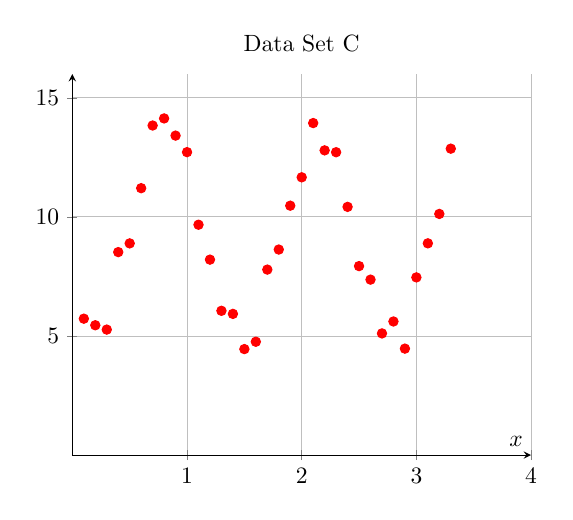
\begin{tikzpicture}[scale=0.85]
            \begin{axis}[axis lines=center, xmin=0, xmax=4, ymin=0, ymax=16, grid,
                xlabel={$x$}, title={Data Set C}]
                \addplot[only marks, mark=*, red] coordinates{
(0.1,5.726977149)
(0.2,5.451391016)
(0.3,5.268948381)
(0.4,8.522301974)
(0.5,8.888857507)
(0.6,11.20634597)
(0.7,13.83745495)
(0.8,14.13499226)
(0.9,13.41374698)
(1,12.7198408)
(1.1,9.671884968)
(1.2,8.206222419)
(1.3,6.057714947)
(1.4,5.928402975)
(1.5,4.450516096)
(1.6,4.758844484)
(1.7,7.788150805)
(1.8,8.629901355)
(1.9,10.471519)
(2,11.6626857)
(2.1,13.94041078)
(2.2,12.79412449)
(2.3,12.71650125)
(2.4,10.42173634)
(2.5,7.934935177)
(2.6,7.366601573)
(2.7,5.108323902)
(2.8,5.609689017)
(2.9,4.470001691)
(3,7.460556729)
(3.1,8.890990059)
(3.2,10.12523049)
(3.3,12.86572276)};
            \end{axis}
        \end{tikzpicture}
    \end{center}
    \caption{Several data plots for Problem \ref{prob:least_squares_plots}.}
    \label{fig:plot_least_squares_prob}
\end{figure}

It should be clear to the reader at this point that curve fitting is actually an
optimization problem.  For every collection of parameters in your chosen function there is
a unique sum of square errors.  The goal, of course, is to pick parameters that minimize
the sum of square errors.  It is beyond the scope of this book to write a gradient
descent or derivative free optimization routine to do this optimization.  Instead we will
lean on several pre-built tools that can do this optimization for us: MS Excel's Solver
and 
\ifnum\Python=0 MATLAB's \texttt{fminsearch}
\else
Python's \texttt{scipy.optimize.fmin}
\fi
to name two of them.  If you are curious about how the
optimization occurs see a course in mathematical optimization or machine learning.

\begin{problem}
    In Problem \ref{prob:least_squares_plots} you made hypotheses about the types of
    functions that fit the data shown in \ref{fig:plot_least_squares_prob}.  Use Excel's
    Solver function to minimize the sum of the square residuals for between your
    parameterized function and the data.  
\end{problem}

\begin{problem}
    Repeat the previous problem with 
    \ifnum\Python=0 MATLAB's \texttt{fminsearch}
    \else
    Python's \texttt{scipy.optimize.fmin}
    \fi
    function.
\end{problem}

\begin{problem}
    With your partner come up with an algebraic function governed by several parameters.
    Add some random noise to your function and then save the data (without any formulas).
    Give your data to a different group in the class and have them reverse engineer your
    function from your data.  The second group should report the function, the parameters,
    and the sum of the square errors.
\end{problem}





\newpage\section{Exercises}

\subsection{Algorithm Summaries}

\begin{problem}
    Starting from Taylor series prove that 
    \[ f'(x) \approx \frac{f(x+h) - f(x)}{h} \]
    is a first-order approximation of the first derivative of $f(x)$.  Clearly describe
    what ``first-order approximation'' means in this context.
\end{problem}

\begin{problem}
    Starting from Taylor series prove that 
    \[ f'(x) \approx \frac{f(x+h) - f(x-h)}{2h} \]
    is a second-order approximation of the first derivative of $f(x)$.  Clearly describe
    what ``second-order approximation'' means in this context.
\end{problem}

\begin{problem}
    Starting from Taylor series prove that 
    \[ f''(x) \approx \frac{f(x+h) - 2f(x) + f(x-h)}{h^2} \]
    is a second-order approximation of the second derivative of $f(x)$.  Clearly describe
    what ``second-order approximation'' means in this context.
\end{problem}

\begin{problem}
    Explain how to approximate the value of a definite integral with Riemann sums.  When
    will the Riemann sum approximation be exact?  The Riemann sum approximation is first
    order.  Expain what ``first order'' means for calculating a definite integral. 
\end{problem}

\begin{problem}
    Explain how to approximate the value of a definite integral with the Trapezoid rule.
    When will the Trapezoid rule approximation be exact?  The Trapezoidal rule
    approximation is second
    order.  Expain what ``second order'' means for calculating a definite integral. 
\end{problem}

\begin{problem}
    Explain how to approximate the value of a definite integral with Simpson's rule.  Give
    the full mathematical details for where Simpson's rule comes from.  When will the
    Simpson's rule approximation be exact?  The Simpson's rule approximation is fourth
    order.  Expain what ``fourth order'' means for calculating a definite integral. 
\end{problem}

\begin{problem}
    Explain in clear language how the derivative free optimization method works on a
    single-variable function.
\end{problem}

\begin{problem}
    Explain in clear language how the gradient descent/ascent optimization method works on a
    single-variable function.
\end{problem}

\begin{problem}
    Explain in clear language how the Monte Carlo search optimization method works on a
    single-variable function.
\end{problem}

\begin{problem}
    Explain in clear language how you find the optimal set of parameters given a set of
    data and a proposed general function type.
\end{problem}

\subsection{Applying What You've Learned}

\begin{problem}
    For each of the following numerical differentiation formulas (1) prove that the
    formula is true and (2) find the order of the method. To prove that each of the
    formulas is true you will need to write the Taylor series for all of the terms in the
    numerator on the right and then simplify to solve for the necessary derivative.  The
    highest power of the remainder should reveal the order of the method.  It would be
    very wise to redo problems \ref{prob:numdiff1} - \ref{prob:num_diff_first_order},
    \ref{prob:numdiff3}, and \ref{prob:numdiff4} before beginning this problem.
    \begin{enumerate}
        \item[(a)] $\ds f'(x) \approx \frac{\frac{1}{12} f(x-2h) - \frac{2}{3} f(x-h) +
            \frac{2}{3} f(x+h) - \frac{1}{12} f(x+2h)}{h}$
        \item[(b)] $\ds f'(x) \approx \frac{-\frac{3}{2} f(x) + 2 f(x+h) -
            \frac{1}{2} f(x+2h)}{h}$
        \item[(c)] $\ds f''(x) \approx \frac{-\frac{1}{12} f(x-2h) + \frac{4}{3} f(x-h) -
            \frac{5}{2} f(x) + \frac{4}{3} f(x+h) - \frac{1}{12} f(x+2h)}{h^2}$
        \item[(d)] $\ds f'''(x) \approx \frac{-\frac{1}{2} f(x-2h) + f(x-h) - f(x+h) +
            \frac{1}{2} f(x+2h)}{h^3}$
    \end{enumerate}
\end{problem}
\hint{
   Let's look at the first one.  If we write the Taylor series for $f(x-2h)$, $f(x-h)$,
   $f(x+h)$, and for $f(x+2h)$ and then form the linear combination suggested in the
   numerator we should be able to solve for $f'(x)$.
   \begin{flalign*}
       f(x-2h) &= f(x) - 2h f'(x) + \frac{4h^2}{2!} f''(x) - \frac{8h^3}{3!} f'''(x) + \cdots
       \\
       f(x-h) &= f(x) - h f'(x) + \frac{h^2}{2!} f''(x) - \frac{h^3}{3!} f'''(x) + \cdots
       \\
       f(x+h) &= f(x) + h f'(x) + \frac{h^2}{2!} f''(x) + \frac{h^3}{3!} f'''(x) + \cdots
       \\
       f(x+2h) &= f(x) + 2h f'(x) + \frac{4h^2}{2!} f''(x) + \frac{8h^3}{3!} f'''(x) + \cdots 
   \end{flalign*}
   Therefore, the linear combination $\frac{1}{12} f(x-2h) - \frac{2}{3} f(x-h) + \frac{2}{3} f(x+h) -
   \frac{1}{12} f(x+2h)$ clearly cancels the $f(x)$ term, leaves $h f'(x)$, cancels the
   $f''(x)$ term, and leaves $h^3 f'''(x)$ multiplied by some non-zero constant.  Solving
   for $f'(x)$ leaves
   \[ f'(x) = \frac{1}{h} \left( \frac{1}{12}f(x-2h) - \frac{2}{3} f(x-h) +
   \frac{2}{3} f(x+h)  - \frac{1}{12} f(x+2h) \right) + \mathcal{O}(h^2), \]
   and we see that this is a second order method since the remainder is on the order of
   $h^2$.
}

\begin{problem}\label{prob:first_deriv_data}
    Write a \ProgLang function that accepts a list of $(x,y)$ ordered pairs from an Excel
    spreadsheet and returns a list of $(x,y)$ ordered pairs for a first order
    approximation of the first derivative of the
    underlying function. 
%     \\
%     \mcode{function [new_x,dydx] = FirstDerivFromData(ExcelFileName,Xrange,Yrange)} \\
%     In the function all of the inputs are strings.  For example \\
%     \mcode{FirstDerivativeFromData('MyFunctionData.xlsx','A2:A101','B2:B101')}\\
    Create a test Excel file and a test script that have graphical output showing that
    your \ProgLang function is finding the correct derivative.
\end{problem}
\hint{
    Be sure to re-define the list of $x$ values so you can plot the output.  You're doing
    this since you are losing information when taking a first derivative.
}



\begin{problem}
    Write a \ProgLang function that accepts a list of $(x,y)$ ordered pairs from an Excel
    spreadsheet and returns a list of $(x,y)$ ordered pairs for a second order
    approximation of the second derivative of the
    underlying function. 
%     \\
%     \mcode{function [new_x,dydx] = SecondDerivFromData(ExcelFileName,Xrange,Yrange)} \\
%     In the function all of the inputs are strings.  For example \\
%     \mcode{SecondDerivativeFromData('MyFunctionData.xlsx','A2:A101','B2:B101')}\\
    Create a test Excel file and a test script that have graphical output showing that
    your \ProgLang function is finding the correct derivative.
\end{problem}
\hint{
    Be sure to re-define the list of $x$ values so you can plot the output.  You're doing
    this since you are losing information when taking a second derivative.
}


\begin{problem}\label{prob:trap_from_data}
    Write a \ProgLang function that implements the trapezoidal rule on a list of $(x,y)$
    order pairs representing the integrand function.  The list of ordered pairs should be
    read from an Excel file. 
%     \\
%     \mcode{function Area = TrapezoidFromData(ExcelFilename, Xlist, Ylist)}\\
%     In the function all of the inputs are strings.  For example \\
%     \mcode{Area = TrapezoidFromData('MyFunctionData.xlsx','A2:A101','B2:B101')}\\
    Create a test Excel file and a test script showing that your \ProgLang function is
    finding the correct integral.
\end{problem}

\begin{problem}
    Use numerical integration to answer the question in each of the following scenarios
    \begin{enumerate}
        \item[(a)] We measure the rate at which water is flowing out of a reservoir (in
            gallons per second) several times over the course of one hour.  Estimate the
            total amount of water which left the reservoir during that hour.
            \begin{center}
                \begin{tabular}{|l||c|c|c|c|c|c|c|}
                    \hline
                    time (min) & 0 & 7 & 19 & 25 & 38 & 47 & 55 \\ \hline
                    flow rate (gal/sec) & 316 & 309 & 296 & 298 & 305 & 314 & 322 \\ \hline
                \end{tabular}
            \end{center}
        \item[(b)] The department of transportation finds that the rate at which cars
            cross a bridge can be approximated by the function
            \[ f(t) = \frac{22.8 }{3.5 + 7(t-1.25)^4} , \]
            where $t=0$ at 4pm, and is measured in hours, and $f(t)$ is measured in cars
            per minute.  Estimate the total number of
            cars that cross the bridge between 4 and 6pm.  Make sure that your estimate has
            an error less than 5\% and provide sufficient mathematical evidence of your
            error estimate.
    \end{enumerate}
\end{problem}


\begin{problem}
    Consider the integrals 
    \[ \int_{-2}^2 e^{-x^2/2} dx \quad \text{and} \quad \int_0^1 \cos(x^2) dx. \]
    Neither of these integrals have closed-form solutions so a numerical method is
    necessary.  Create a loglog plot that shows the errors for the integrals with different values of $h$ (log
    of $h$ on the $x$-axis and log of the absolute error on the $y$-axis).
    Write a complete interpretation of the loglog plot.  
    To get the {\it exact} answer for these plots use the 
    \ifnum\Python=0 MATLAB \mcode{quad} command.
    \else
    Python's \texttt{scipy.integrate.quad} command.
    \fi
    (What we're really doing here is comparing our algorithms to \ProgLang's built in algorithm).
\end{problem}


\begin{problem}
    Go to \href{https://www.data.gov/}{data.gov} or the
    \href{http://apps.who.int/gho/data/?theme=home}{World Health Organization Data
    Repository} and find data sets for the following tasks.
    \begin{enumerate}
        \item[(a)] Find a data set where the variables naturally lead to a meaningful
            derivative.  Use your code from Problem  \ref{prob:first_deriv_data} to
            evaluate and plot the derivative.  If your data appears to be subject to
            significant noise then use the Excel curve fitting tools first to smooth the
            data; then do the derivative.  Write a few sentences explaning what the
            derivative means in the context of the data.
        \item[(b)] Find a data set where the variables naturally lead to a meaningfun
            definite integral.  Use your code from Problem \ref{prob:trap_from_data} to
            evaluate the definite integral.  If your data appears to be subject to
            significant noise then use the Excel curve fitting tools first to smooth the
            data; then do the integral.  Write a few sentences explaning what the
            integral means in the context of the data.
    \end{enumerate}
    In both of these tasks be very cautious of the units on the data sets and the units of
    your answer. 
\end{problem}

% \begin{problem}
%     Go to the \href{http://apps.who.int/gho/data/?theme=home}{World Health Organization
%     Data Repository} and find a data set where it would make physical sense to integrate
%     (and that the integral would tell you something meaningful about the data).  Use your
%     MATLAB code to take the integral and provide context and meaning associated with the
%     integral.  You will need to download the data as a CSV or Excel file and import the
%     proper columns into Excel (Google \texttt{xlsread} to learn how MATLAB imports Excel
%     data). Your data set will obviously involved some noise, but one thought might be to
%     find a data set that shows a trend in time.
% \end{problem}




\begin{problem}
    Integrate each of the functions over the interval $[-1,2]$ and verify mathematically
    that your numerical integral is correct to 10 decimal places.  Then provide a plot of
    the function along with its numerical first derivative.
    \begin{enumerate}
        \item[(a)] $\ds f(x) = \frac{x}{1+x^4}$
        \item[(b)] $\ds g(x) = (x-1)^3 (x-2)^2$
        \item[(c)] $\ds h(x) = \sin\left(x^2\right)$
    \end{enumerate}
\end{problem}


\begin{problem}
    A bicyclist completes a race course in 90 seconds.  The speed of the biker at each
    10-second interval is determined using a radar gun and is given in the table in feet
    per second.  How long is the race course?
    \begin{center}
        \begin{tabular}{|c||c|c|c|c|c|c|c|c|c|c|}
            \hline
            Time (sec) &      0 & 10 & 20 & 30 & 40 & 50 & 60 & 70 & 80 & 90 \\ \hline
            Speed (ft/sec) & 34 & 32 & 29 & 33 & 37 & 40 & 41 & 36 & 38 & 39 \\
            \hline
        \end{tabular}
        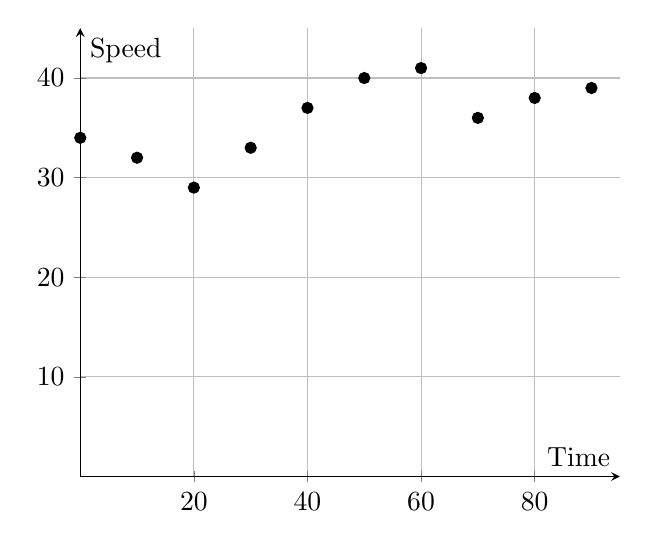
\begin{tikzpicture}
            \begin{axis}[axis lines=center, grid, xlabel={Time}, ylabel={Speed}, ymin=0,
                ymax=45, xmin=0, xmax=95]
                \addplot[only marks, mark=*] coordinates{
(0,34)(10,32)(20,29)(30,33)(40,37)(50,40)(60,41)(70,36)(80,38)(90,39)
                };
            \end{axis}
        \end{tikzpicture}
    \end{center}
\end{problem}

\begin{problem}
    For each of the following functions write code to find the local maximum or minimum
    that is closest to $x=0$.  You may want to start with a plot of the function just to
    get a feel for where the local extreme value might be.
    \begin{enumerate}
        \item[(a)] $\displaystyle f(x) = \frac{x}{1+x^4} + \sin(x)$
        \item[(b)] $\displaystyle g(x) =
            \left(x-1\right)^3\cdot\left(x-2\right)^2+e^{-0.5\cdot x}$
    \end{enumerate}
\end{problem}

\begin{problem}
    Go back to your old Calculus textbook or homework and find your favorite optimization
    problem.  State the problem, create the mathematical model, and use any of the numerical
    optimization techniques in this chapter to get an approximate solution to the problem.
\end{problem}


% \begin{problem}
%     Although Simpson’s rule was derived from parabolas, prove that it integrates all cubic
%     polynomials exactly.
% \end{problem}
% \hint{
%     Apply Simpson's rule to the function $f(x) = Ax^3 + Bx^2 + Cx + D$ on the interval
%     $[\alpha,\beta]$. This means that you will be evaluating the function at $\alpha$,
%     $\beta$, and $(\alpha+\beta)/2$. You can also easily do this integral by hand
%     symbolically:
%     \[ \int_\alpha^\beta Ax^3 + Bx^2 + Cx + D dx = \left( \frac{Ax^4}{4} + \frac{Bx^3}{3} +
%     \frac{Cx^2}{2} + Dx \right) \Big|_{\alpha}^{\beta} = \cdots. \]
%     Verify that
%     Simpson's rule gives exactly the same answer symbolically.
% 
% 
% 
% }


\begin{problem}\label{prob:curve_fitting_exercises}
    The plots in Figure \ref{fig:curve_fitting_exercises_plots} show noisy data from
    measurements of elementary single variable functions.
    \begin{enumerate}
        \item[(a)] Make a hypothesis about which function would best model the data.  Be
            sure to choose the most general (parameterized) form of your function.
        \item[(b)] Use appropriate tools to find the parameters for the function that best
            fits the data.  Report you sum of square residuals for each function.
    \end{enumerate}
    Your instructor will provide you with the raw data.  Note that in the pictures the
    points are connected with line segments simply for visual effect.  The functions that
    you propose must be continuous functions.
\end{problem}

\begin{figure}
    \begin{center}
        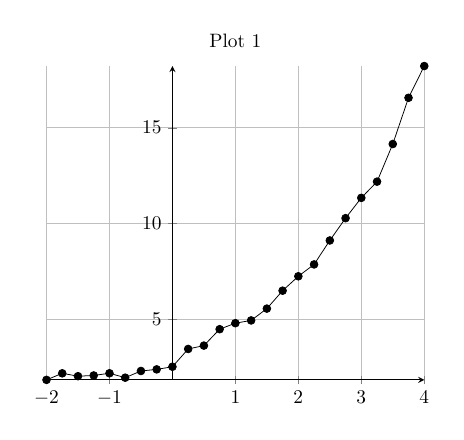
\begin{tikzpicture}[scale=0.7]
            \begin{axis}[axis lines=center, grid, title={Plot 1}]
                \addplot[mark=*] coordinates{
(-2,1.827786408)
(-1.75,2.170530273)
(-1.5,2.019732122)
(-1.25,2.057766355)
(-1,2.17271598)
(-0.75,1.942496758)
(-0.5,2.292477808)
(-0.25,2.375761311)
(0,2.513562722)
(0.25,3.442073414)
(0.5,3.61851248)
(0.75,4.475996146)
(1,4.789748499)
(1.25,4.933434388)
(1.5,5.550603846)
(1.75,6.487375499)
(2,7.240339006)
(2.25,7.86003591)
(2.5,9.11138024)
(2.75,10.27594456)
(3,11.33635172)
(3.25,12.18428112)
(3.5,14.14964853)
(3.75,16.56485404)
(4,18.2238497)};
            \end{axis}
        \end{tikzpicture}
        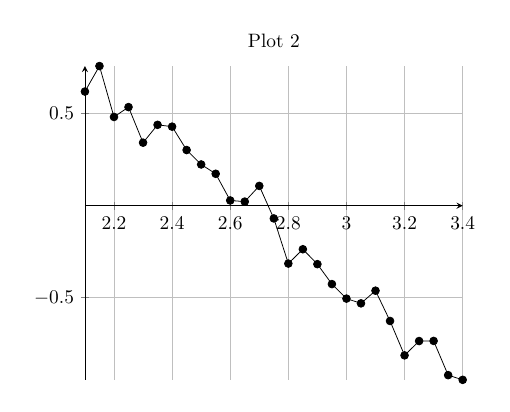
\begin{tikzpicture}[scale=0.7]
            \begin{axis}[axis lines=center, grid, title={Plot 2}]
                \addplot[mark=*] coordinates{
(2.1,0.620338852)
(2.15,0.759019708)
(2.2,0.482214049)
(2.25,0.53588217)
(2.3,0.34247563)
(2.35,0.439417407)
(2.4,0.429595117)
(2.45,0.302408858)
(2.5,0.223982914)
(2.55,0.173392192)
(2.6,0.028261824)
(2.65,0.021951597)
(2.7,0.107375196)
(2.75,-0.069410942)
(2.8,-0.314749946)
(2.85,-0.236846404)
(2.9,-0.317968664)
(2.95,-0.426385845)
(3,-0.505269643)
(3.05,-0.531048933)
(3.1,-0.462195205)
(3.15,-0.626844591)
(3.2,-0.813851088)
(3.25,-0.735954667)
(3.3,-0.735269866)
(3.35,-0.921349293)
(3.4,-0.946931813)};
            \end{axis}
        \end{tikzpicture}
        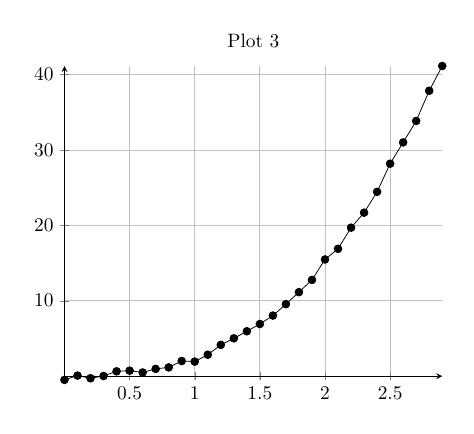
\begin{tikzpicture}[scale=0.7]
            \begin{axis}[axis lines=center, grid, title={Plot 3}]
                \addplot[mark=*] coordinates{
(0,-0.49450467)
(0.1,0.074882224)
(0.2,-0.280201153)
(0.3,0.018639459)
(0.4,0.639046545)
(0.5,0.727185342)
(0.6,0.485092813)
(0.7,0.963801405)
(0.8,1.159105789)
(0.9,2.008918263)
(1,1.930847198)
(1.1,2.843770713)
(1.2,4.143790566)
(1.3,5.014551507)
(1.4,5.952787591)
(1.5,6.913618934)
(1.6,8.03577976)
(1.7,9.551625656)
(1.8,11.13870628)
(1.9,12.76217261)
(2,15.47325475)
(2.1,16.88943329)
(2.2,19.69117887)
(2.3,21.68001629)
(2.4,24.44268896)
(2.5,28.17440543)
(2.6,30.99558273)
(2.7,33.84180928)
(2.8,37.84754694)
(2.9,41.12278565)};
            \end{axis}
        \end{tikzpicture}
        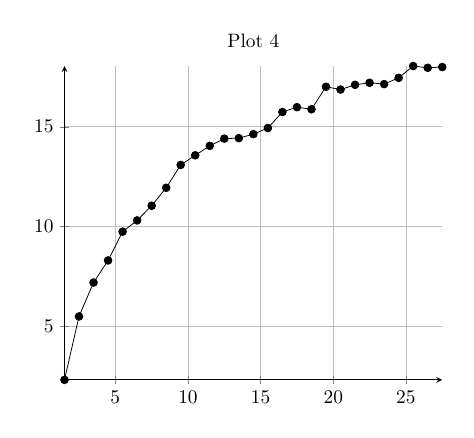
\begin{tikzpicture}[scale=0.7]
            \begin{axis}[axis lines=center, grid, title={Plot 4}]
                \addplot[mark=*] coordinates{
(1.5,2.31155657)
(2.5,5.491397071)
(3.5,7.190096486)
(4.5,8.297376083)
(5.5,9.741290241)
(6.5,10.30523328)
(7.5,11.0397925)
(8.5,11.94081088)
(9.5,13.08619213)
(10.5,13.56793153)
(11.5,14.04205556)
(12.5,14.40464555)
(13.5,14.42870765)
(14.5,14.62766086)
(15.5,14.93646003)
(16.5,15.73757069)
(17.5,15.98043913)
(18.5,15.87607647)
(19.5,17.00392144)
(20.5,16.8631223)
(21.5,17.10052368)
(22.5,17.20283334)
(23.5,17.13711573)
(24.5,17.45093371)
(25.5,18.04228498)
(26.5,17.95394595)
(27.5,17.99192879)};
            \end{axis}
        \end{tikzpicture}
        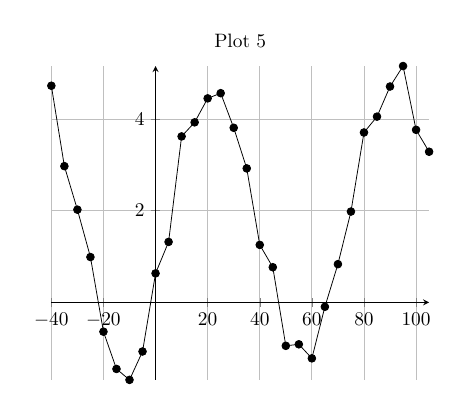
\begin{tikzpicture}[scale=0.7]
            \begin{axis}[axis lines=center, grid, title={Plot 5}]
                \addplot[mark=*] coordinates{
(-40,4.724118031)
(-35,2.970593363)
(-30,2.022103405)
(-25,0.988760498)
(-20,-0.638952765)
(-15,-1.451314878)
(-10,-1.689669505)
(-5,-1.070830009)
(0,0.632982269)
(5,1.318823566)
(10,3.619200845)
(15,3.926166409)
(20,4.448776279)
(25,4.562237908)
(30,3.807258343)
(35,2.922016094)
(40,1.253764377)
(45,0.766680021)
(50,-0.947218851)
(55,-0.913895463)
(60,-1.220299677)
(65,-0.095971864)
(70,0.833611733)
(75,1.980746366)
(80,3.7049767)
(85,4.050528706)
(90,4.707082482)
(95,5.153787151)
(100,3.762765979)
(105,3.285155548)};
            \end{axis}
        \end{tikzpicture}
        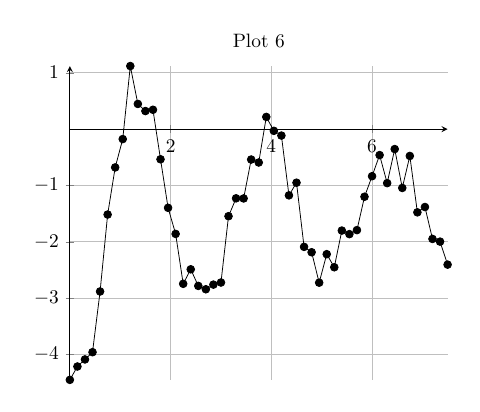
\begin{tikzpicture}[scale=0.7]
            \begin{axis}[axis lines=center, grid, title={Plot 6}]
                \addplot[mark=*] coordinates{
(0.00,-4.449456854)
(0.15,-4.212500338)
(0.30,-4.086912168)
(0.45,-3.958253448)
(0.60,-2.881162505)
(0.75,-1.516197323)
(0.90,-0.68014595)
(1.05,-0.177100517)
(1.20,1.118573477)
(1.35,0.44615688)
(1.50,0.320134332)
(1.65,0.342550908)
(1.80,-0.535494042)
(1.95,-1.397032043)
(2.10,-1.859736685)
(2.25,-2.745103944)
(2.40,-2.488002665)
(2.55,-2.782439112)
(2.70,-2.841948189)
(2.85,-2.75955687)
(3.00,-2.722051195)
(3.15,-1.545683776)
(3.30,-1.228319356)
(3.45,-1.230759993)
(3.60,-0.540113141)
(3.75,-0.592703675)
(3.90,0.215782074)
(4.05,-0.031060909)
(4.20,-0.115011378)
(4.35,-1.175832922)
(4.50,-0.951259528)
(4.65,-2.08979662)
(4.80,-2.18517115)
(4.95,-2.725035231)
(5.10,-2.219480806)
(5.25,-2.45141889)
(5.40,-1.800646406)
(5.55,-1.86379778)
(5.70,-1.792482425)
(5.85,-1.200554602)
(6.00,-0.835991703)
(6.15,-0.46111166)
(6.30,-0.958544571)
(6.45,-0.354479352)
(6.60,-1.044511886)
(6.75,-0.476860167)
(6.90,-1.477006626)
(7.05,-1.382719845)
(7.20,-1.948987485)
(7.35,-1.996719751)
(7.50,-2.404790592)
                };
            \end{axis}
        \end{tikzpicture}
        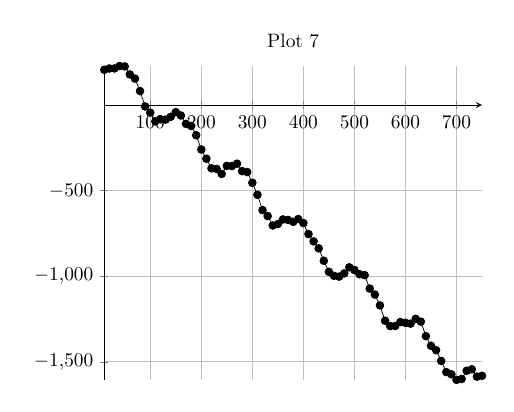
\begin{tikzpicture}[scale=0.7]
            \begin{axis}[axis lines=center, grid, title={Plot 7}]
                \addplot[mark=*] coordinates{
(10,206.0162568)
(20,213.4795786)
(30,213.8403229)
(40,227.802522)
(50,225.6197982)
(60,178.7024779)
(70,154.6892911)
(80,81.70057476)
(90,-8.290132861)
(100,-44.3517702)
(110,-95.36553972)
(120,-83.44395348)
(130,-85.20228987)
(140,-69.12110337)
(150,-41.58994093)
(160,-61.22638559)
(170,-110.0814716)
(180,-122.2322317)
(190,-176.5522583)
(200,-259.8652098)
(210,-313.825314)
(220,-369.8081213)
(230,-373.4277422)
(240,-402.7449841)
(250,-355.602077)
(260,-356.3934396)
(270,-342.7772839)
(280,-386.4015738)
(290,-391.7199628)
(300,-454.393317)
(310,-524.6232437)
(320,-614.1378148)
(330,-648.8071556)
(340,-703.8465558)
(350,-695.5106182)
(360,-668.7108834)
(370,-671.599177)
(380,-682.674601)
(390,-666.2483273)
(400,-689.8332274)
(410,-753.9896633)
(420,-796.7433458)
(430,-837.4518064)
(440,-909.9882962)
(450,-974.8774748)
(460,-998.042244)
(470,-1002.693716)
(480,-984.0242486)
(490,-948.3226958)
(500,-964.1660252)
(510,-988.8113091)
(520,-994.1954627)
(530,-1072.776731)
(540,-1107.559613)
(550,-1170.933896)
(560,-1260.422949)
(570,-1291.672619)
(580,-1291.217712)
(590,-1268.269071)
(600,-1272.855738)
(610,-1277.466874)
(620,-1249.499903)
(630,-1265.720551)
(640,-1350.556404)
(650,-1406.935395)
(660,-1432.828131)
(670,-1495.389775)
(680,-1560.88485)
(690,-1573.797742)
(700,-1606.136223)
(710,-1600.866859)
(720,-1552.632809)
(730,-1544.440208)
(740,-1587.076728)
(750,-1582.311195)
                };
            \end{axis}
        \end{tikzpicture}
        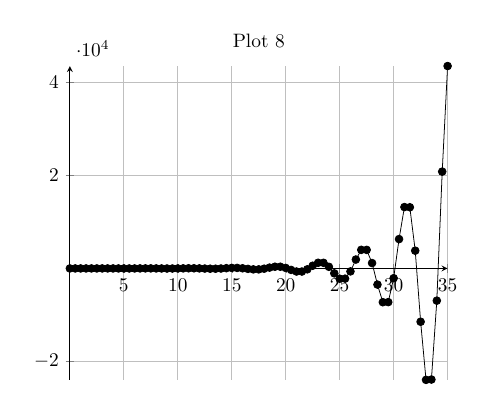
\begin{tikzpicture}[scale=0.7]
            \begin{axis}[axis lines=center, grid, title={Plot 8}]
                \addplot[mark=*] coordinates{
(0.0,0.659805301)
(0.5,-0.415972824)
(1.0,-1.093474007)
(1.5,-1.249873742)
(2.0,0.395555473)
(2.5,1.597684532)
(3.0,3.399269869)
(3.5,3.362888296)
(4.0,0.959267282)
(4.5,-1.844324035)
(5.0,-5.044155285)
(5.5,-4.903557845)
(6.0,-1.279140485)
(6.5,5.424622027)
(7.0,11.22472144)
(7.5,10.60573166)
(8.0,3.089113846)
(8.5,-8.380206751)
(9.0,-18.584297)
(9.5,-17.57421137)
(10.0,-4.636727794)
(10.5,16.70714519)
(11.0,34.61943853)
(11.5,34.08552591)
(12.0,9.999537095)
(12.5,-28.4617782)
(13.0,-61.08782039)
(13.5,-61.18615294)
(14.0,-17.08638893)
(14.5,53.43805698)
(15.0,112.0812828)
(15.5,112.1685705)
(16.0,32.51571344)
(16.5,-96.36121442)
(17.0,-201.8196697)
(17.5,-201.9570412)
(18.0,-57.87079944)
(18.5,176.8096134)
(19.0,368.4821508)
(19.5,366.9361248)
(20.0,106.9307101)
(20.5,-318.9581464)
(21.0,-667.3899625)
(21.5,-665.4839399)
(22.0,-192.7005797)
(22.5,581.542834)
(23.0,1214.089857)
(23.5,1210.65027)
(24.0,351.9569967)
(24.5,-1054.078092)
(25.0,-2203.468422)
(25.5,-2197.234689)
(26.0,-636.8994402)
(26.5,1915.326131)
(27.0,4003.513699)
(27.5,3992.263187)
(28.0,1158.068478)
(28.5,-3477.726226)
(29.0,-7269.851302)
(29.5,-7248.790785)
(30.0,-2101.934685)
(30.5,6317.854301)
(31.0,13205.51654)
(31.5,13166.34932)
(32.0,3819.087971)
(32.5,-11472.95664)
(33.0,-23982.027)
(33.5,-23910.41909)
(34.0,-6934.694149)
(34.5,20838.7478)
(35.0,43557.86423)
                };
            \end{axis}
        \end{tikzpicture}
    \end{center}
    \caption{Plots for Problem \ref{prob:curve_fitting_exercises}.}
    \label{fig:curve_fitting_exercises_plots}
\end{figure}




\newpage\section{Projects}
In this section we propose several ideas for projects related to numerical Calculus.  These
projects are meant to be open ended, to encourage creative mathematics, to push your
coding skills, and to require you to write and communicate your mathematics.  Take the
time to read Appendix \ref{app:writing_projects} before you write your final solution.


\subsection{Galaxy Integration}

To analyze the light from stars and galaxies, scientists use a spectral grating (fancy prism) to
split it up into the different frequencies (colors). We can then measure the intensity
(brightness) of the light (in units of Watts per square meter) at each frequency (measured
in Hertz), to get intensity per frequency (Watts per square meter per Hertz, W/(m$^2$
Hz)). Light from the dense opaque surface of a star produces a smooth rainbow, which
produces a continuous curve when we plot intensity versus frequency. However stars are
also surrounded by thin gas which either emits or absorbs light at only a specific set of
frequencies, called spectral lines. Every chemical element produces a specific set of
lines (or peaks) at fixed frequencies, so by identifying the lines, we can tell what types of atoms
and molecules a star is made of. If the gas is cool, then it will absorb light at these
wavelengths, and if the gas is hot then it will emit light at these wavelengths. For
galaxies, on the other hand, we expect mostly emission spectra: light emitted from the
galaxy.  

For this project we will be analyzing the galaxy ``ngc 1275''.  The black hole at the
center of this galaxy is often referred to as the ``Galactic Spaghetti Monster'' since the magnetic field ``sustains a mammoth network of
spaghetti-like gas filaments around it''.\footnote{\href{https://www.newscientist.com/article/dn14573-galactic-spaghetti-monster-powered-by-magnetic-fields/}{www.newscientist.com/article/dn14573-galactic-spaghetti-monster-powered-by-magnetic-fields/}}
% 
In the Excel file associated with this project you will see the spectral data measuring the
light intensity from ncg 1275 at several different wavelengths (measured in Angstroms
).
You will notice in this data set that there are several emission lines at various
wavelengths.  Of particular interest are the peaks near
$3800$ Angstroms, $5100$ Angstroms, $6400$ Angstroms, and the two peaks around $6700$ Angstroms. The data
set contains 1,727 data points at different wavelengths. Your first job will be to
transform the wavelength data to frequency via the formula
\[ \lambda = \frac{c}{f} \]
where $\lambda$ is the wavelength, $c$ is the speed of light, and $f$ is the frequency
(measured in Hertz). Be sure to double check the units. Given the inverse relationship
between frequency and wavelength you should see the emission lines flip to the other side
of the plot (right-to-left or left-to-right).  


The strength of each emission line (in W/m$^2$) is defined as the relative intensity of each peak
\underline{integrated}
across the associated frequencies. Note that you are not interested in the intensity of the continuous
spectrum -- just the peaks. That is to say that you are only interested in the area above
the background curve and the background noise.  

% \subsection*{Your Tasks}
Your primary task is to develop a process
for analyzing data sets like this so as to determine the strength of each emission lines.
You must demonstrate your process on this particular data set, but your process must be
generalizable to any similar data set.
Your process must clearly 
determine the strength of peaks in data sets like this and you must apply your procedure
to determine the strength of each of these four lines with an associated margin of
error.\footnote{I would be surprised if you didn't do some statistics along the way.}
Keep in mind that you will first want to first develop a method for removing the
background noise. Finally, the double peak near $6700$ Angstroms needs to be handled with care:
the strength of each emission line is only the integral over one peak, not two, so you'll
need to determine a way to separate these peaks.

Finally, it would be cool, but is not necessary, to report on which chemicals
correspond to the emission lines in the data.  Remember that the galaxy is far away and
hence there is a non-trivial red-shift to consider.  This will take some research but if
done properly will likely give a lot more merit to your paper.

\subsection{Higher Order Integration}
Riemann sums can be used to approximate integrals and they do so by using piecewise
constant functions to approximate the function.  The trapezoidal rule uses piecewise
linear functions to approximate the function and then the area of a trapezoid to
approximate the area.  We saw earlier that Simpson's rule uses piecewise parabolas to
approximate the function.  The process which we used to build Simpson's rule can be
extended to any higher-order polynomial.  Your job in this project is to build integration
algorithms that use piecewise cubic functions, quartic functions, etc.  For each you need
to show all of the mathematics necessary to derive the algorithm, provide several test
cases to show that the algorithm works, and produce a numerical experiment that shows the
order of accuracy of the algorithm.  

\subsection{Dam Integration}
Go to the USGS water data repository: \\
\href{https://maps.waterdata.usgs.gov/mapper/index.html}{https://maps.waterdata.usgs.gov/mapper/index.html}.\\
Here you'll find a map with information about water resources around the country.
\begin{itemize}
    \item Zoom in to a dam of your choice (make sure that it is a dam).
    \item Click on the map tag then click ``Access Data''
    \item From the dropdown menu at the top select either ``Daily Data'' or ``Current
        / Historical Data''.  If these options don't appear then choose a different
        dam.
    \item Change the dates so you have the past year's worth of information.
    \item Select ``Tab-separated'' under ``Output format'' and press Go.  Be sure that
        the data you got has a flow rate (ft$^3$/sec).
    \item At this point you should have access to the entire data set.  Copy it into a
        \texttt{csv} file and save it to your computer.
\end{itemize}
For the data that you just downloaded you have three tasks: (1) plot the data in a
reasonable way giving appropriate units, (2) find the total amount of water that
has been discharged from the dam during the past calendar year, and (3) report any
margin of error in your calculation based on the numerical method that you used in
part (2).

